\begin{minipage}[b]{0.33\linewidth}
\begin{lrbox}{\mybox}%
\begin{lstlisting}[basicstyle=\ttfamily\tiny]
* = $0801
;---------------------------------
; Start program at InitializeProgram
; SYS 2064 ($0810)
;---------------------------------
 .BYTE $0B,$08
 .BYTE $C1,$07
 .BYTE $9E
 .BYTE $32,$30,$36,$34
 .BYTE $00
 .BYTE $00,$00
 .BYTE $F9,$02,$F9


;------------------------------
; InitializeProgram
;------------------------------
InitializeProgram
 LDA #$00
 STA $D020
 STA $D021

 JSR MovePresetDataIntoPosition

 STA previousIndexToPixelBuffers

 LDA #>COLOR_RAM
 STA colorRamHiPtr
 LDA #<COLOR_RAM
 STA colorRamLoPtr

 LDX #$00
InitColorRamTableLoop
 LDA colorRamHiPtr
 STA colorRAMLineTableHiPtrArray,X
 LDA colorRamLoPtr
 STA colorRAMLineTableLoPtrArray,X
 CLC
 ADC #NUM_COLS
 STA colorRamLoPtr
 LDA colorRamHiPtr
 ADC #$00
 STA colorRamHiPtr
 INX
 CPX #NUM_ROWS + 1
 BNE InitColorRamTableLoop

 LDA #$80
 STA $0291

 LDA #$15
 STA $D018

 JSR ROM_IOINIT
 JSR InitializeDynamicStorage
 JMP LaunchPsychedelia

colorRAMLineTableLoPtrArray
 .BYTE $00,$00,$00,$00,$00,$00,$00,$00
 .BYTE $00,$00,$00,$00,$00,$00,$00,$00
 .BYTE $00,$00,$00,$00,$00,$00,$00,$00
 .BYTE $00,$00,$00,$00,$00,$00
colorRAMLineTableHiPtrArray
 .BYTE $00,$00,$00,$00,$00,$00,$BF,$00
 .BYTE $00,$00,$00,$00,$00,$00,$00,$00
 .BYTE $00,$00,$00,$00,$00,$00,$00,$00
 .BYTE $00,$00,$00,$00,$00,$00

;------------------------------
; InitializeScreenWithInitCharacter
;------------------------------
InitializeScreenWithInitCharacter
 LDX #$00

currentPixel = *+$01
InitScreenLoop
 LDA #$CF
 STA SCREEN_RAM + $0000,X
 STA SCREEN_RAM + $0100,X
 STA SCREEN_RAM + $0200,X
 STA SCREEN_RAM + $02C0,X
 LDA #$00
 STA COLOR_RAM + $0000,X
 STA COLOR_RAM + $0100,X
 STA COLOR_RAM + $0200,X
 STA COLOR_RAM + $02C0,X
 DEX
 BNE InitScreenLoop
 RTS

presetKeyCodes
 .BYTE KEY_LEFT,KEY_1,KEY_2,KEY_3
 .BYTE KEY_4,KEY_5,KEY_6,KEY_7
 .BYTE KEY_8,KEY_9,KEY_0,KEY_PLUS
 .BYTE KEY_MINUS,KEY_POUND
 .BYTE KEY_CLR_HOME,KEY_INST_DEL

;------------------------------
; LoadXAndYPosition
;------------------------------
LoadXAndYPosition
 LDX pixelYPosition
 LDA colorRAMLineTableLoPtrArray,X
 STA currentLineInColorRamLoPtr2
 LDA colorRAMLineTableHiPtrArray,X
 STA currentLineInColorRamHiPtr2
 LDY pixelXPosition
ReturnEarlyFromRoutine
 RTS
\end{lstlisting}
\end{lrbox}%
\scalebox{0.8}{\usebox{\mybox}}
\end{minipage}
\hspace{-0.1cm}
\begin{minipage}[b]{0.33\linewidth}
\begin{lrbox}{\mybox}%
\begin{lstlisting}[basicstyle=\ttfamily\tiny]
;------------------------------
; PaintPixel
;------------------------------
PaintPixel
 LDA pixelXPosition
 AND #$80
 BNE ReturnEarlyFromRoutine
 LDA pixelXPosition
 CMP #NUM_COLS
 BPL ReturnEarlyFromRoutine
 LDA pixelYPosition
 AND #$80
 BNE ReturnEarlyFromRoutine
 LDA pixelYPosition
 CMP #NUM_ROWS
 BPL ReturnEarlyFromRoutine

 JSR LoadXAndYPosition
 LDA skipPixel
 BNE ActuallyPaintPixel

 LDA (currentLineInColorRamLoPtr2),Y
 AND #COLOR_MAX

 LDX #$00
GetIndexInPresetsLoop
 CMP presetColorValuesArray,X
 BEQ FoundMatchingIndex
 INX
 CPX #COLOR_VALUES_ARRAY_LEN
 BNE GetIndexInPresetsLoop

FoundMatchingIndex
 TXA
 STA indexOfCurrentColor
 LDX currentValueInColorIndexArray
 INX
 CPX indexOfCurrentColor
 BEQ ActuallyPaintPixel
 BPL ActuallyPaintPixel
 RTS

ActuallyPaintPixel
 LDX currentValueInColorIndexArray
 LDA presetColorValuesArray,X
 STA (currentLineInColorRamLoPtr2),Y
 RTS

;------------------------------
; PaintStructureAtCurrentPosition
;------------------------------
PaintStructureAtCurrentPosition
 JSR PaintPixelForCurrentSymmetry
 LDY #$00
 LDA currentValueInColorIndexArray
 CMP #NUM_ARRAYS
 BNE CanLoopAndPaint
 RTS

CanLoopAndPaint
 LDA #NUM_ARRAYS
 STA countToMatchCurrentIndex

 LDA pixelXPosition
 STA previousPixelXPosition
 LDA pixelYPosition
 STA previousPixelYPosition

 LDX patternIndex
 LDA pixelXPositionLoPtrArray,X
 STA xPosLoPtr
 LDA pixelXPositionHiPtrArray,X
 STA xPosHiPtr
 LDA pixelYPositionLoPtrArray,X
 STA yPosLoPtr
 LDA pixelYPositionHiPtrArray,X
 STA yPosHiPtr

PixelPaintLoop
 LDA previousPixelXPosition
 CLC
 ADC (xPosLoPtr),Y
 STA pixelXPosition
 LDA previousPixelYPosition
 CLC
 ADC (yPosLoPtr),Y
 STA pixelYPosition

 TYA
 PHA
 JSR PaintPixelForCurrentSymmetry
 PLA
 TAY
 INY

 LDA (xPosLoPtr),Y
 CMP #$55
 BNE PixelPaintLoop

 DEC countToMatchCurrentIndex
 LDA countToMatchCurrentIndex
 CMP currentValueInColorIndexArray
 BEQ RestorePositionsAndReturn

 CMP #$01
 BEQ RestorePositionsAndReturn

 INY
 JMP PixelPaintLoop
\end{lstlisting}
\end{lrbox}%
\scalebox{0.8}{\usebox{\mybox}}
\end{minipage}
\hspace{-0.1cm}
\begin{minipage}[b]{0.33\linewidth}
\begin{lrbox}{\mybox}%
\begin{lstlisting}[basicstyle=\ttfamily\tiny]
RestorePositionsAndReturn
 LDA previousPixelXPosition
 STA pixelXPosition
 LDA previousPixelYPosition
 STA pixelYPosition
 RTS

;        5       
;                
;       4 4      
;        3       
;        2       
;        1       
;   4   000   4  
; 5  3210 0123  5
;   4   000   4  
;        1       
;        2       
;        3       
;       4 4      
;                
;        5       
starOneXPosArray  
.BYTE $00,$01,$01,$01,$00
.BYTE $FF,$FF,$FF,$55
.BYTE $00,$02,$00,$FE,$55
.BYTE $00,$03,$00,$FD,$55
.BYTE $00,$04,$00,$FC,$55
.BYTE $FF,$01,$05,$05,$01
.BYTE $FF,$FB,$FB,$55
.BYTE $00,$07,$00,$F9,$55
.BYTE $55
starOneYPosArray  
.BYTE $FF,$FF,$00,$01,$01
.BYTE $01,$00,$FF,$55
.BYTE $FE,$00,$02,$00,$55
.BYTE $FD,$00,$03,$00,$55
.BYTE $FC,$00,$04,$00,$55
.BYTE $FB,$FB,$FF,$01,$05
.BYTE $05,$01,$FF,$55
.BYTE $F9,$00,$07,$00,$55
.BYTE $55

countToMatchCurrentIndex   .BYTE $00

;------------------------------
; PutRandomByteInAccumulator
;------------------------------
PutRandomByteInAccumulator
randomByteAddress   =*+$01
 LDA $E199,X
 INC randomByteAddress
 RTS

;------------------------------
; PaintPixelForCurrentSymmetry
;------------------------------
PaintPixelForCurrentSymmetry
 LDA pixelXPosition
 PHA
 LDA pixelYPosition
 PHA
 JSR PaintPixel

 LDA currentSymmetrySettingForStep
 BNE HasSymmetry

CleanUpAndReturnFromSymmetry
 PLA
 STA pixelYPosition
 PLA
 STA pixelXPosition
 RTS

HasSymmetry
 CMP #X_AXIS_SYMMETRY
 BEQ XAxisSymmetry

 LDA #NUM_COLS - 1
 SEC
 SBC pixelXPosition
 STA pixelXPosition

 LDY currentSymmetrySettingForStep
 CPY #X_Y_SYMMETRY
 BEQ XYSymmetry

 JSR PaintPixel

 LDA currentSymmetrySettingForStep
 CMP #Y_AXIS_SYMMETRY
 BEQ CleanUpAndReturnFromSymmetry

 LDA #NUM_ROWS - 1
 SEC
 SBC pixelYPosition
 STA pixelYPosition
 JSR PaintPixel

PaintXAxisPixelForSymmetry
 PLA
 TAY
 PLA
 STA pixelXPosition
 TYA
 PHA
 JSR PaintPixel
 PLA
 STA pixelYPosition
 RTS

\end{lstlisting}
\end{lrbox}%
\scalebox{0.8}{\usebox{\mybox}}
\end{minipage}
\clearpage
\rhead[]{The Core of the Game on a Page or Two}
\textbf{Lines 1 - 710.} This first section is almost exactly the same as its equivalent in the listing. On this
page and the following two we have the core of the game from which the version we saw in 
\hyperref[sec:commentary]{\textcolor{blue}{'let's pretend we can read code'}} was carved out.

What this tells us, I think, is that what we have here and in the following two pages represents the very initial state
of Psychedelia when it was first developed: 

\begin{definition}[Jeffrey Says]
\setlength{\intextsep}{0pt}%
\setlength{\columnsep}{3pt}%
\begin{wrapfigure}{l}{0.12\textwidth}

\includegraphics[width=\linewidth]{src/callout/psych.png} 
\end{wrapfigure}
\small
.. one day I was out running and an just appeared unbidden in my head. I still
  remember the exact bit of road I was on when it happened. It was a
  simple algorithm, just seeding patterns along a path; the patterns were to
  expand and change shape and colour over time. I got back from my run and
  coded up the algo - it fit in about 1K of 6502 assembler code. I ran the code
  and a white cursor appeared on the screen. i picked up the joystick, moved
  the cursor, and pressed down the fire button.

In that instant my life changed.
\end{definition}

So this three pages of code is the product of an evening's work - the nucleus of the game as a whole. The fact that among
the code we have a single data structure for a single pattern reinforces this notion: a simple demo neededed just one
pattern to work with, so there it is, propped between \icode{PaintStructureAtCurrentPosition} and \icode{PaintPixelForCurrentSymmetry}.

Once the basic demo was working, it was time to add some more patterns and we can see these inserted after the interrupt handler
code in the final column on the following pages: 'The Twist', 'La Llamita', and 'Star Two' make their appearance.

The writing of a complete game was underway.

\clearpage
\begin{minipage}[b]{0.33\linewidth}
\begin{lrbox}{\mybox}%
\begin{lstlisting}[basicstyle=\ttfamily\tiny]
XAxisSymmetry
 LDA #NUM_ROWS - 1
 SEC
 SBC pixelYPosition
 STA pixelYPosition
 JMP PaintXAxisPixelForSymmetry
XYSymmetry
 LDA #NUM_ROWS - 1
 SEC
 SBC pixelYPosition
 STA pixelYPosition
 JSR PaintPixel
 PLA
 STA pixelYPosition
 PLA
 STA pixelXPosition
 RTS

pixelXPositionArray
 .BYTE $00,$00,$FF,$00,$00,$00,$00,$00
 .BYTE $00,$00,$00,$00,$00,$00,$00,$00
 .BYTE $00,$00,$00,$00,$00,$00,$00,$00
 .BYTE $00,$00,$FF,$00,$00,$00,$00,$00
 .BYTE $00,$00,$00,$00,$00,$00,$00,$00
 .BYTE $00,$00,$00,$00,$00,$00,$00,$00
 .BYTE $00,$00,$00,$00,$00,$00,$00,$00
 .BYTE $00,$00,$00,$00,$00,$00,$00,$00
pixelYPositionArray
 .BYTE $00,$00,$FD,$00,$00,$00,$00,$00
 .BYTE $00,$00,$00,$00,$00,$00,$00,$00
 .BYTE $00,$00,$00,$00,$00,$00,$00,$00
 .BYTE $00,$00,$00,$00,$00,$00,$00,$00
 .BYTE $00,$00,$00,$00,$00,$00,$00,$00
 .BYTE $00,$00,$00,$00,$00,$00,$00,$00
 .BYTE $00,$00,$00,$00,$00,$00,$00,$00
 .BYTE $00,$00,$00,$00,$00,$00,$00,$00
currentColorIndexArray
 .BYTE $00,$00,$00,$00,$00,$00,$00,$00
 .BYTE $00,$00,$00,$00,$00,$00,$00,$00
 .BYTE $00,$00,$00,$00,$00,$00,$00,$00
 .BYTE $00,$00,$00,$00,$00,$00,$00,$00
 .BYTE $00,$00,$00,$00,$00,$00,$00,$00
 .BYTE $00,$00,$00,$00,$00,$00,$00,$00
 .BYTE $00,$00,$00,$00,$00,$00,$00,$00
 .BYTE $00,$00,$00,$00,$00,$00,$00,$00
initialSmoothingDelayArray
 .BYTE $00,$00,$00,$00,$00,$00,$00,$00
 .BYTE $00,$00,$00,$00,$00,$00,$00,$00
 .BYTE $00,$00,$00,$00,$00,$00,$00,$00
 .BYTE $00,$00,$FF,$FF,$FF,$FF,$FF,$FF
 .BYTE $FF,$FF,$FF,$FF,$FF,$FF,$FF,$FF
 .BYTE $FF,$FF,$FF,$FF,$FF,$FF,$FF,$FF
 .BYTE $FF,$FF,$FF,$FF,$FF,$FF,$FF,$FF
 .BYTE $FF,$FF,$FF,$FF,$FF,$FF,$FF,$FF
smoothingDelayArray
 .BYTE $FF,$FF,$FF,$FF,$FF,$FF,$FF,$FF
 .BYTE $FF,$FF,$FF,$FF,$FF,$FF,$FF,$FF
 .BYTE $FF,$FF,$FF,$FF,$FF,$FF,$FF,$FF
 .BYTE $FF,$FF,$FF,$FF,$FF,$FF,$FF,$FF
 .BYTE $FF,$FF,$FF,$FF,$FF,$FF,$FF,$FF
 .BYTE $FF,$FF,$FF,$FF,$FF,$FF,$FF,$FF
 .BYTE $FF,$FF,$FF,$FF,$FF,$FF,$FF,$FF
 .BYTE $FF,$FF,$FF,$FF,$FF,$FF,$FF,$FF
patternIndexArray
 .BYTE $FF,$FF,$FF,$FF,$FF,$FF,$FF,$FF
 .BYTE $FF,$FF,$FF,$FF,$FF,$FF,$FF,$FF
 .BYTE $FF,$FF,$FF,$FF,$FF,$FF,$FF,$FF
 .BYTE $FF,$FF,$FF,$FF,$FF,$FF,$FF,$FF
 .BYTE $FF,$FF,$FF,$FF,$FF,$FF,$FF,$FF
 .BYTE $FF,$FF,$FF,$FF,$FF,$FF,$FF,$FF
 .BYTE $FF,$FF,$FF,$FF,$FF,$FF,$FF,$FF
 .BYTE $FF,$FF,$FF,$FF,$FF,$FF,$FF,$FF
symmetrySettingForStepCount
 .BYTE $FF,$FF,$FF,$FF,$FF,$FF,$FF,$FF
 .BYTE $FF,$FF,$FF,$FF,$FF,$FF,$FF,$FF
 .BYTE $FF,$FF,$FF,$FF,$FF,$FF,$FF,$FF
 .BYTE $FF,$FF,$FF,$FF,$FF,$FF,$FF,$FF
 .BYTE $FF,$FF,$FF,$FF,$FF,$FF,$FF,$FF
 .BYTE $FF,$FF,$FF,$FF,$FF,$FF,$FF,$FF
 .BYTE $FF,$FF,$FF,$FF,$FF,$FF,$FF,$FF
 .BYTE $FF,$FF,$FF,$FF,$FF,$FF,$FF,$FF

;------------------------------
; ReinitializeSequences
;------------------------------
ReinitializeSequences
 LDX #$00
 TXA
_Loop   
 STA pixelXPositionArray,X
 STA pixelYPositionArray,X
 LDA #$FF
 STA currentColorIndexArray,X
 LDA #$00
 STA initialSmoothingDelayArray,X
 STA smoothingDelayArray,X
 STA patternIndexArray,X
 STA symmetrySettingForStepCount,X
 INX
 CPX #PIXEL_BUFFER_LENGTH
 BNE _Loop
 STA timerBetweenKeyStrokes
 STA currentPatternElement
 STA previousIndexToPixelBuffers
 STA skipPixel
 LDA #Y_AXIS_SYMMETRY
 STA currentSymmetrySetting
 RTS
\end{lstlisting}
\end{lrbox}%
\scalebox{0.8}{\usebox{\mybox}}
\end{minipage}
\hspace{-0.1cm}
\begin{minipage}[b]{0.33\linewidth}
\begin{lrbox}{\mybox}%
\begin{lstlisting}[basicstyle=\ttfamily\tiny]
;------------------------------
; LaunchPsychedelia
;------------------------------
LaunchPsychedelia
 JSR SetUpInterruptHandlers

 LDX #$10
_Loop   TXA
 STA SetUpInterruptHandlers,X
 DEX
 BNE _Loop

 JSR ReinitializeScreen
 JSR ReinitializeSequences
 JSR ClearLastLineOfScreen

;------------------------------
; MainPaintLoop
;------------------------------
MainPaintLoop
 INC currentIndexToPixelBuffers

 LDA lastKeyPressed
 CMP #KEY_CRSR_LEFT_RIGHT
 BNE HandleAnyCurrentModes

_Loop   LDA lastKeyPressed
 CMP #NO_KEY_PRESSED
 BNE _Loop

_Loop2  LDA lastKeyPressed
 CMP #KEY_CRSR_LEFT_RIGHT
 BNE _Loop2

_Loop3  LDA lastKeyPressed
 CMP #NO_KEY_PRESSED
 BNE _Loop3

HandleAnyCurrentModes
 LDA currentModeActive
 BEQ DoANormalPaint

 CMP #CUSTOM_PRESET_MODE_ACTIVE
 BNE MaybeInSavePromptMode

 JMP HandleCustomPreset

MaybeInSavePromptMode
 CMP #SAVE_PROMPT_MODE_ACTIVE
 BNE InitializeScreenAndPaint
 JMP DisplaySavePromptScreen

InitializeScreenAndPaint
 JSR ReinitializeScreen

DoANormalPaint
 LDA currentIndexToPixelBuffers
 CMP bufferLength
 BNE CheckCurrentBuffer

 LDA #$00
 STA currentIndexToPixelBuffers
CheckCurrentBuffer
 LDX currentIndexToPixelBuffers
 LDA currentColorIndexArray,X
 CMP #$FF
 BNE ShouldDoAPaint

 STX previousIndexToPixelBuffers
 JMP MainPaintLoop

ShouldDoAPaint
 STA currentValueInColorIndexArray
 DEC smoothingDelayArray,X
 BNE GoBackToStartOfLoop


 LDA initialSmoothingDelayArray,X
 STA smoothingDelayArray,X

 LDA pixelXPositionArray,X
 STA pixelXPosition
 LDA pixelYPositionArray,X
 STA pixelYPosition

 LDA patternIndexArray,X
 STA patternIndex

 LDA symmetrySettingForStepCount,X
 STA currentSymmetrySettingForStep

 LDA currentValueInColorIndexArray
 AND #LINE_MODE_ACTIVE
 BNE PaintLineModeAndLoop

 TXA
 PHA
 JSR PaintStructureAtCurrentPosition
 PLA
 TAX

 DEC currentColorIndexArray,X
GoBackToStartOfLoop
 JMP MainPaintLoop

currentIndexToPixelBuffers   .BYTE $00
PaintLineModeAndLoop
 JMP PaintLineMode
\end{lstlisting}
\end{lrbox}%
\scalebox{0.8}{\usebox{\mybox}}
\end{minipage}
\hspace{-0.1cm}
\begin{minipage}[b]{0.33\linewidth}
\begin{lrbox}{\mybox}%
\begin{lstlisting}[basicstyle=\ttfamily\tiny]
;------------------------------
; SetUpInterruptHandlers
;------------------------------
SetUpInterruptHandlers
 SEI
 LDA #<MainInterruptHandler
 STA $0314
 LDA #>MainInterruptHandler
 STA $0315

 LDA #$0A
 STA cursorXPosition
 STA cursorYPosition

 LDA #$01
 STA $D015
 STA $D027

 LDA #<NMIInterruptHandler
 STA $0318
 LDA #>NMIInterruptHandler
 STA $0319
 CLI
 RTS

countStepsBeforeCheckingJoystick   
.BYTE $02,$00
;------------------------------
; MainInterruptHandler
;------------------------------
MainInterruptHandler
 LDA stepsRemainingInSequencerSequence
 BEQ SequencerNotActiveCheckJoystick
 DEC stepsRemainingInSequencerSequence
 BNE SequencerNotActiveCheckJoystick

 LDA sequencerSpeed
 STA stepsRemainingInSequencerSequence

CalledFromNMI
 JSR LoadDataForSequencer

SequencerNotActiveCheckJoystick
 DEC countStepsBeforeCheckingJoystick
 BEQ CanUpdatePixelBuffers

 JMP CheckKeyboardAndExitInterrupt

CanUpdatePixelBuffers
 LDA #BLACK
 STA currentColorToPaint
 LDA cursorSpeed
 STA countStepsBeforeCheckingJoystick
 JSR PaintCursorAtCurrentPosition

 JSR GetJoystickInput
 LDA lastJoystickInput
 AND #JOYSTICK_UP | JOYSTICK_DOWN
 CMP #JOYSTICK_UP | JOYSTICK_DOWN
 BEQ CheckIfCursorMovedLeftOrRight

 CMP #JOYSTICK_DOWN
 BEQ PlayerHasPressedDown

 INC cursorYPosition
 INC cursorYPosition

PlayerHasPressedDown
 DEC cursorYPosition
 LDA cursorYPosition

 CMP #BELOW_ZERO
 BNE CheckIfCursorAtBottom

 LDA #NUM_ROWS - 1
 STA cursorYPosition
 JMP CheckIfCursorMovedLeftOrRight

CheckIfCursorAtBottom
 CMP #NUM_ROWS
 BNE CheckIfCursorMovedLeftOrRight
 LDA #$00
 STA cursorYPosition

CheckIfCursorMovedLeftOrRight
 LDA lastJoystickInput
 AND #JOYSTICK_RIGHT | JOYSTICK_LEFT
 CMP #JOYSTICK_RIGHT | JOYSTICK_LEFT
 BEQ CheckIfPlayerPressedFire

 CMP #JOYSTICK_RIGHT
 BEQ CursorMovedLeft

 INC cursorXPosition
 INC cursorXPosition

CursorMovedLeft
 DEC cursorXPosition
 LDA cursorXPosition
 CMP #BELOW_ZERO
 BNE CheckIfCursorAtExtremeRight

 LDA #NUM_COLS - 1
 STA cursorXPosition
 JMP CheckIfPlayerPressedFire
CheckIfCursorAtExtremeRight
 CMP #NUM_COLS
 BNE CheckIfPlayerPressedFire
\end{lstlisting}
\end{lrbox}%
\scalebox{0.8}{\usebox{\mybox}}
\end{minipage}
\begin{minipage}[b]{0.33\linewidth}
\begin{lrbox}{\mybox}%
\begin{lstlisting}[basicstyle=\ttfamily\tiny]
 LDA #$00
 STA cursorXPosition
CheckIfPlayerPressedFire
 LDA lastJoystickInput
 AND #$10
 BEQ PlayerHasPressedFire

 LDA #$00
 STA stepsSincePressedFire
 JMP DrawCursorAndReturnFromInterrupt

PlayerHasPressedFire
 LDA stepsExceeded255
 BEQ DecrementPulseWidthCounter
 LDA stepsSincePressedFire
 BEQ IncrementStepsSincePressedFire
 JMP DrawCursorAndReturnFromInterrupt

IncrementStepsSincePressedFire
 INC stepsSincePressedFire

DecrementPulseWidthCounter
 LDA currentPulseWidth
 BEQ DecrementPulseSpeedCounter
 DEC currentPulseWidth
 BEQ DecrementPulseSpeedCounter
 JMP UpdatePixelBuffersForPattern

DecrementPulseSpeedCounter
 DEC currentPulseSpeedCounter
 BEQ RefreshPulseSpeed
 JMP DrawCursorAndReturnFromInterrupt

RefreshPulseSpeed
 LDA pulseSpeed
 STA currentPulseSpeedCounter
 LDA pulseWidth
 STA currentPulseWidth

UpdatePixelBuffersForPattern
 INC currentStepCount
 LDA currentStepCount
 CMP bufferLength
 BNE UpdateBaseLevelArray

 LDA #$00
 STA currentStepCount

UpdateBaseLevelArray
 TAX
 LDA currentColorIndexArray,X
 CMP #$FF
 BEQ UpdatePositionArrays

 LDA previousIndexToPixelBuffers
 AND trackingActivated
 BEQ DrawCursorAndReturnFromInterrupt

 TAX
 LDA currentColorIndexArray,X
 CMP #$FF
 BNE DrawCursorAndReturnFromInterrupt

 STX currentStepCount

UpdatePositionArrays
 LDA cursorXPosition
 STA pixelXPositionArray,X
 LDA cursorYPosition
 STA pixelYPositionArray,X

 LDA lineModeActivated
 BEQ LineModeNotActive

 LDA #NUM_ROWS + 1
 SEC
 SBC cursorYPosition
 ORA #$80
 STA currentColorIndexArray,X

 JMP ApplySmoothingDelay

LineModeNotActive
 LDA baseLevel
 STA currentColorIndexArray,X
 LDA currentPatternElement
 STA patternIndexArray,X

ApplySmoothingDelay
 LDA smoothingDelay
 STA initialSmoothingDelayArray,X
 STA smoothingDelayArray,X
 LDA currentSymmetrySetting
 STA symmetrySettingForStepCount,X

DrawCursorAndReturnFromInterrupt
 LDA #WHITE
 STA currentColorToPaint
 JSR PaintCursorAtCurrentPosition

;------------------------------
; CheckKeyboardAndExitInterrupt
;------------------------------
CheckKeyboardAndExitInterrupt
 JSR CheckKeyboardInput
 JMP RETURN_INTERRUPT
\end{lstlisting}
\end{lrbox}%
\scalebox{0.8}{\usebox{\mybox}}
\end{minipage}
\hspace{-0.1cm}
\begin{minipage}[b]{0.33\linewidth}
\begin{lrbox}{\mybox}%
\begin{lstlisting}[basicstyle=\ttfamily\tiny]
;------------------------------
; LoadXAndYOfCursorPosition
;------------------------------
LoadXAndYOfCursorPosition
 LDX cursorYPosition
 LDA colorRAMLineTableLoPtrArray,X
 STA currentLineInColorRamLoPtr

 LDA colorRAMLineTableHiPtrArray,X
 STA currentLineInColorRamHiPtr

 LDY cursorXPosition
ReturnEarlyFromCursorPaint
 RTS

;------------------------------
; PaintCursorAtCurrentPosition
;------------------------------
PaintCursorAtCurrentPosition
 LDA displaySavePromptActive
 BNE ReturnEarlyFromCursorPaint

 JSR LoadXAndYOfCursorPosition
 LDA currentColorToPaint
 STA (currentLineInColorRamLoPtr),Y

 RTS

cursorXPosition       .BYTE $0A
cursorYPosition       .BYTE $0A
currentStepCount      .BYTE $00
stepsSincePressedFire .BYTE $00
stepsExceeded255      .BYTE $00

presetValueArray
unusedPresetByte        .BYTE $00
smoothingDelay          .BYTE $0C
cursorSpeed             .BYTE $02
bufferLength            .BYTE $1F
pulseSpeed              .BYTE $01
indexForColorBarDisplay .BYTE $01
lineWidth               .BYTE $07
sequencerSpeed          .BYTE $04
pulseWidth              .BYTE $01
baseLevel               .BYTE $07

presetColorValuesArray
.BYTE BLACK,BLUE,RED,PURPLE
.BYTE GREEN,CYAN,YELLOW,WHITE
trackingActivated       .BYTE $FF
lineModeActivated       .BYTE $00
patternIndex            .BYTE $05

pixelXPositionLoPtrArray
.BYTE <starOneXPosArray,<theTwistXPosArray,<laLlamitaXPosArray
.BYTE <starTwoXPosArray,<deltoidXPosArray,<diffusedXPosArray
.BYTE <multicrossXPosArray,<pulsarXPosArray

customPatternLoPtrArray
.BYTE <customPattern0XPosArray,<customPattern1XPosArray
.BYTE <customPattern2XPosArray,<customPattern3XPosArray
.BYTE <customPattern4XPosArray,<customPattern5XPosArray
.BYTE <customPattern6XPosArray,<customPattern7XPosArray

pixelXPositionHiPtrArray
.BYTE >starOneXPosArray,>theTwistXPosArray,>laLlamitaXPosArray
.BYTE >starTwoXPosArray,>deltoidXPosArray,>diffusedXPosArray
.BYTE >multicrossXPosArray,>pulsarXPosArray

customPatternHiPtrArray
.BYTE >customPattern0XPosArray,>customPattern1XPosArray
.BYTE >customPattern2XPosArray,>customPattern3XPosArray
.BYTE >customPattern4XPosArray,>customPattern5XPosArray
.BYTE >customPattern6XPosArray,>customPattern7XPosArray

pixelYPositionLoPtrArray
.BYTE <starOneYPosArray,<theTwistYPosArray,<laLlamitaYPosArray
.BYTE <starTwoYPosArray,<deltoidYPosArray,<diffusedYPosArray
.BYTE <multicrossYPosArray,<pulsarYPosArray
.BYTE <customPattern0YPosArray,<customPattern1YPosArray
.BYTE <customPattern2YPosArray,<customPattern3YPosArray

\end{lstlisting}
\end{lrbox}%
\scalebox{0.8}{\usebox{\mybox}}
\end{minipage}
\hspace{-0.1cm}
\begin{minipage}[b]{0.33\linewidth}
\begin{lrbox}{\mybox}%
\begin{lstlisting}[basicstyle=\ttfamily\tiny]
.BYTE <customPattern4YPosArray,<customPattern5YPosArray
.BYTE <customPattern6YPosArray,<customPattern7YPosArray

pixelYPositionHiPtrArray
.BYTE >starOneYPosArray,>theTwistYPosArray,>laLlamitaYPosArray
.BYTE >starTwoYPosArray,>deltoidYPosArray,>diffusedYPosArray
.BYTE >multicrossYPosArray,>pulsarYPosArray
.BYTE >customPattern0YPosArray,>customPattern1YPosArray
.BYTE >customPattern2YPosArray,>customPattern3YPosArray
.BYTE >customPattern4YPosArray,>customPattern5YPosArray
.BYTE >customPattern6YPosArray,>customPattern7YPosArray


;     1  
;   01   
;  6 222 
;  543   
; 5 4 3  
;   4  3 
;       3
theTwistXPosArray
.BYTE $00,$55
.BYTE $01,$02,$55
.BYTE $01,$02,$03,$55
.BYTE $01,$02,$03,$04,$55
.BYTE $00,$00,$00,$55
.BYTE $FF,$FE,$55
.BYTE $FF,$55
.BYTE $55

theTwistYPosArray
.BYTE $FF,$55
.BYTE $FF,$FE,$55
.BYTE $00,$00,$00,$55
.BYTE $01,$02,$03,$04,$55
.BYTE $01,$02,$03,$55
.BYTE $01,$02,$55
.BYTE $00,$55
.BYTE $55



;  0      
; 06      
;  0      
;  1    3 
;  12223 3
;  22223  
;  333 4  
;  4   4  
; 54  54  
laLlamitaXPosArray
.BYTE $00,$FF,$00,$55
.BYTE $00,$00,$55
.BYTE $01,$02,$03,$00,$01,$02,$03,$55
.BYTE $04,$05,$06,$04,$00,$01,$02,$55
.BYTE $04,$00,$04,$00,$04,$55
.BYTE $FF,$03,$55
.BYTE $00,$55

laLlamitaYPosArray
.BYTE $FF,$00,$01,$55
.BYTE $02,$03,$55
.BYTE $03,$03,$03,$04,$04,$04,$04,$55
.BYTE $03,$02,$03,$04,$05,$05,$05,$55
.BYTE $05,$06,$06,$07,$07,$55
.BYTE $07,$07,$55
.BYTE $00,$55



;    1  
;   0  2
;    6  
; 4     
;     3 
;  5    
starTwoXPosArray
.BYTE $FF,$55
.BYTE $00,$55
.BYTE $02,$55
.BYTE $01,$55
.BYTE $FD,$55
.BYTE $FE,$55
.BYTE $00,$55

starTwoYPosArray  
.BYTE $FF,$55
.BYTE $FE,$55
.BYTE $FF,$55
.BYTE $02,$55
.BYTE $01,$55
.BYTE $FC,$55
.BYTE $00,$55

\end{lstlisting}
\end{lrbox}%
\scalebox{0.8}{\usebox{\mybox}}
\end{minipage}
\begin{minipage}[b]{0.33\linewidth}
\begin{lrbox}{\mybox}%
\begin{lstlisting}[basicstyle=\ttfamily\tiny]
;       5      
;              
;       4      
;       3      
;       2      
;      202     
;     20602    
;    3     3   
;   4       4  
;              
; 5           5
deltoidXPosArray
.BYTE $00,$01,$FF,$55
.BYTE $00,$55
.BYTE $00,$01,$02,$FE,$FF,$55
.BYTE $00,$03,$FD,$55
.BYTE $00,$04,$FC,$55
.BYTE $00,$06,$FA,$55
.BYTE $00,$55

deltoidYPosArray
.BYTE $FF,$00,$00,$55
.BYTE $00,$55
.BYTE $FE,$FF,$00,$00,$FF,$55
.BYTE $FD,$01,$01,$55
.BYTE $FC,$02,$02,$55
.BYTE $FA,$04,$04,$55
.BYTE $00,$55



; 5            
;            4 
;   3          
;          2   
; 5   1       5
;   3    0  3  
;       6      
;   3  0    3  
; 5       1   5
;    2         
;           3  
;  4           
;             5
diffusedXPosArray
.BYTE $FF,$01,$55
.BYTE $FE,$02,$55
.BYTE $FD,$03,$55
.BYTE $FC,$04,$FC,$FC,$04,$04,$55
.BYTE $FB,$05,$55
.BYTE $FA,$06,$FA,$FA,$06,$06,$55
.BYTE $00,$55

diffusedYPosArray
.BYTE $01,$FF,$55
.BYTE $FE,$02,$55
.BYTE $03,$FD,$55
.BYTE $FC,$04,$FF,$01,$FF,$01,$55
.BYTE $05,$FB,$55
.BYTE $FA,$06,$FE,$02,$FE,$02,$55
.BYTE $00,$55




;------------------------------
; CheckKeyboardInput
;------------------------------
CheckKeyboardInput
 LDA currentVariableMode
 BEQ CheckForGeneralKeystrokes
 JMP CheckKeyboardInputForMode

CheckForGeneralKeystrokes
 LDA timerBetweenKeyStrokes
 BEQ CheckForKeyStroke
 DEC timerBetweenKeyStrokes
 BNE ReturnFromKeyboardCheck

CheckForKeyStroke
 LDA lastKeyPressed
 CMP #NO_KEY_PRESSED
 BNE ProcessKeyStroke

 LDA #$00
 STA timerBetweenKeyStrokes
 JSR MaybeDisplayDemoModeMessage
ReturnFromKeyboardCheck
 RTS

ProcessKeyStroke
 LDY initialTimeBetweenKeyStrokes
 STY timerBetweenKeyStrokes
 LDY shiftKey
 STY shiftPressed

 CMP #KEY_SPACE
 BNE MaybeSPressed

 INC currentPatternElement
 LDA currentPatternElement
 AND #$0F
 STA currentPatternElement

 AND #$08
 BEQ UpdateCurrentPattern

 JMP GetCustomPatternElement



\end{lstlisting}
\end{lrbox}%
\scalebox{0.8}{\usebox{\mybox}}
\end{minipage}
\hspace{-0.1cm}
\begin{minipage}[b]{0.33\linewidth}
\begin{lrbox}{\mybox}%
\begin{lstlisting}[basicstyle=\ttfamily\tiny]
UpdateCurrentPattern
 JSR ClearLastLineOfScreen
 LDA currentPatternElement
 ASL
 ASL
 ASL
 ASL
 TAY

 LDX #$00
txtPresetLoop
 LDA txtPresetPatternNames,Y
 STA statusLineBuffer,X

 INY
 INX
 CPX #DISPLAY_LINE_LENGTH
 BNE txtPresetLoop
 JMP WriteLastLineBufferToScreen

MaybeSPressed
 CMP #KEY_S
 BNE MaybeLPressed

 LDA shiftPressed
 AND #SHIFT_PRESSED
 BEQ JustSPressed

 LDA tapeSavingInProgress
 BNE JustSPressed
 JMP PromptToSave

JustSPressed
 INC currentSymmetrySetting
 LDA currentSymmetrySetting
 CMP #QUAD_SYMMETRY + 1
 BNE DisplaySymmetry

 LDA #$00
 STA currentSymmetrySetting
DisplaySymmetry
 ASL
 ASL
 ASL
 ASL
 TAY
 JSR ClearLastLineOfScreen

 LDX #$00
txtSymmLoop
 LDA txtSymmetrySettingDescriptions,Y
 STA statusLineBuffer,X
 INY
 INX
 CPX #DISPLAY_LINE_LENGTH
 BNE txtSymmLoop

 JMP WriteLastLineBufferToScreen

MaybeLPressed
 CMP #KEY_L
 BNE MaybeDPressed

 LDA tapeSavingInProgress
 BNE JustLPressed

 LDA shiftPressed
 AND #SHIFT_PRESSED
 BEQ JustLPressed

 JMP DisplayLoadOrAbort

JustLPressed
 LDA lineModeActivated
 EOR #$01
 STA lineModeActivated
 ASL
 ASL
 ASL
 ASL
 TAY

 JSR ClearLastLineOfScreen
 LDX #$00
_Loop
 LDA lineModeSettingDescriptions,Y
 STA statusLineBuffer,X
 INY
 INX
 CPX #DISPLAY_LINE_LENGTH
 BNE _Loop
 JMP WriteLastLineBufferToScreen

MaybeDPressed
 CMP #KEY_D
 BNE MaybeCPressed

 LDA #SMOOTHING_DELAY
 STA currentVariableMode
 RTS

MaybeCPressed
 CMP #KEY_C
 BNE MaybeBPressed

 LDA #CURSOR_SPEED
 STA currentVariableMode
 RTS

\end{lstlisting}
\end{lrbox}%
\scalebox{0.8}{\usebox{\mybox}}
\end{minipage}
\hspace{-0.1cm}
\begin{minipage}[b]{0.33\linewidth}
\begin{lrbox}{\mybox}%
\begin{lstlisting}[basicstyle=\ttfamily\tiny]
MaybeBPressed
 CMP #KEY_B
 BNE MaybePPressed

 LDA #BUFFER_LENGTH
 STA currentVariableMode
 RTS

MaybePPressed
 CMP #KEY_P
 BNE MaybeHPressed

 LDA #PULSE_SPEED
 STA currentVariableMode
 RTS

MaybeHPressed
 CMP #KEY_H
 BNE MaybeTPressed

 LDA #$01
 STA currentColorSet
 LDA #COLOR_CHANGE
 STA currentVariableMode
 RTS

MaybeTPressed
 CMP #KEY_T
 BNE CheckIfPresetKeysPressed

 LDA trackingActivated
 EOR #$FF
 STA trackingActivated

 AND #$01
 ASL
 ASL
 ASL
 ASL
 TAY
 JSR ClearLastLineOfScreen

 LDX #$00
txtTrackingLoop
 LDA txtTrackingOnOff,Y
 STA statusLineBuffer,X

 INY
 INX
 CPX #DISPLAY_LINE_LENGTH
 BNE txtTrackingLoop

 JMP WriteLastLineBufferToScreen
 RTS

CheckIfPresetKeysPressed
 LDX #$00
presetKeyLoop
 CMP presetKeyCodes,X
 BEQ UpdateDisplayedPreset
 INX
 CPX #DISPLAY_LINE_LENGTH
 BNE presetKeyLoop

 JMP MaybeWPressed

UpdateDisplayedPreset
 JMP DisplayPresetMessage

MaybeWPressed
 CMP #KEY_W
 BNE MaybeFunctionKeysPressed

 LDA #LINE_WIDTH
 STA currentVariableMode
 RTS

MaybeFunctionKeysPressed
 LDX #$00
FnKeyLoop
 CMP functionKeys,X
 BEQ FunctionKeyWasPressed

 INX
 CPX #$04
 BNE FnKeyLoop
 JMP MaybeQPressed

FunctionKeyWasPressed
 STX functionKeyIndex
 LDA sequencerActive
 BNE MaybeQPressed
 LDA #SEQUENCER_OR_BURST_ACTIVE
 STA currentVariableMode
 JSR LoadOrProgramBurstGenerator
 RTS


MaybeQPressed
 CMP #KEY_Q
 BNE MaybeVPressed


 LDA sequencerActive
 BNE TurnSequenceOff
 LDA #SEQUENCER_OR_BURST_ACTIVE
 STA currentVariableMode
 JMP ActivateSequencer

\end{lstlisting}
\end{lrbox}%
\scalebox{0.8}{\usebox{\mybox}}
\end{minipage}
\clearpage
\rhead[]{Input, Settings, Admin}
\textbf{Lines 710 - 1643.} With the main business of the game taken care of, it is time to add features and settings.

That means creating a lot of configuration options and allowing the player to set them on or off. This and the following
pages concern themselves entirely with handling user input and acting on it. The monster function starting opposite,
\icode{CheckKeyboardInput}, is run from the interrupt handler and checks for all potential keyboard input from the player,
one key at a time. It runs all the way to the following page and is followed by a couple of new pattern definitions, belying
the incremental nature of development: add a new feature, then add a few more patterns to keep things interesting.

The code that follows implements some of the complicated keyboard interactions such as increasing/decreasing various modes
and color settings. It also looks after programming and loading the burst, sequencer, and preset data which we will cover in the
\hyperref[sec:bursts]{\textcolor{blue}{'beatific bursts'}},
\hyperref[sec:sequencer]{\textcolor{blue}{'sensitive sequencer'}}, and
\hyperref[sec:presets]{\textcolor{blue}{'particular presets'}} chapters.

The sheer volume of code required to manage this overhead is an object lesson that holds true for most forms of software development:
much of our time is spent managing detail ancillary to the main purpose of the program. The core that delivers the magic is always
relatively small and self-contained, making the thing presentable is what generates the bloat and most of the hard labour.

\begin{figure}[H]                                                          
  \centering                                                             
  \begin{adjustbox}{width=8cm,center}                                   
  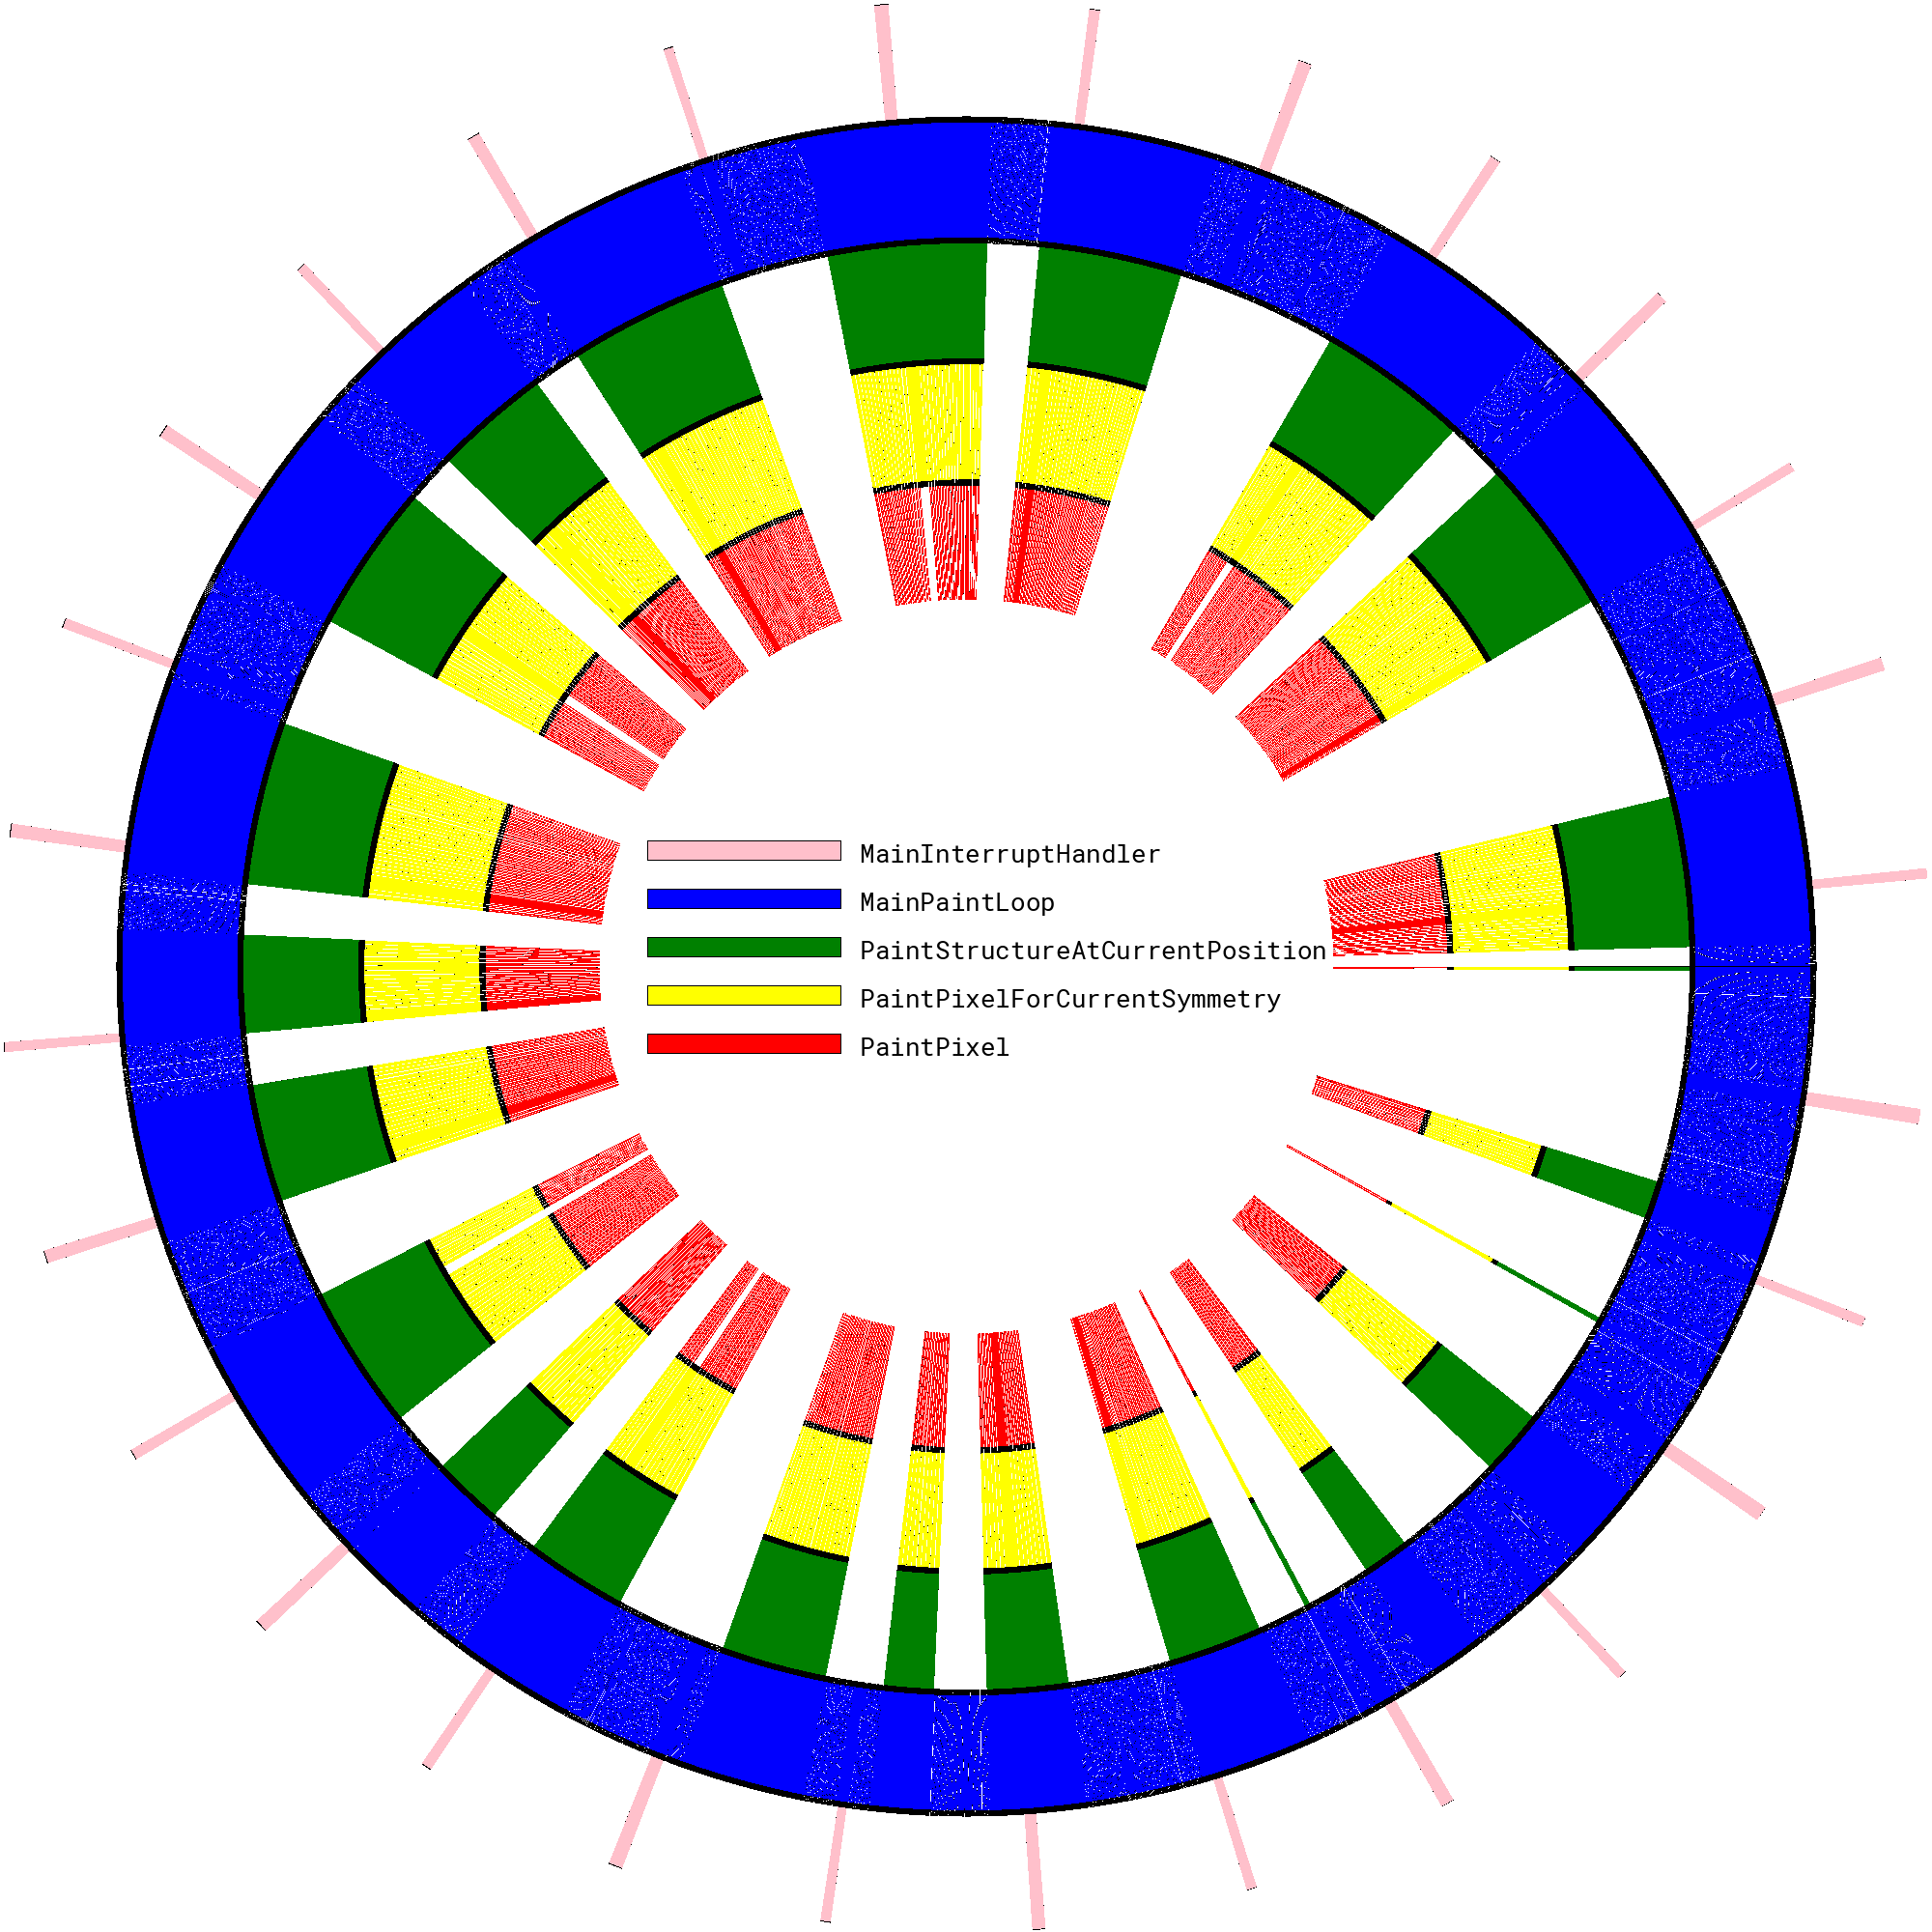
\includegraphics[width=10cm]{src/listing_commentary/execution_cycle.png}%           
  \end{adjustbox}                                                        
\caption{The execution map of a full pattern evolution in the commercial edition of Psychedelia.}                                           
\end{figure}                                                               

\clearpage
\begin{minipage}[b]{0.33\linewidth}
\begin{lrbox}{\mybox}%
\begin{lstlisting}[basicstyle=\ttfamily\tiny]
TurnSequenceOff
 LDA #$00
 STA sequencerActive
 STA stepsRemainingInSequencerSequence
 JMP DisplaySequencerState

MaybeVPressed
 CMP #KEY_V
 BNE MaybeOPressed

 LDA #SEQUENCER_SPEED
 STA currentVariableMode
 RTS

MaybeOPressed
 CMP #KEY_O
 BNE MaybeAsteriskPressed

 LDA #PULSE_WIDTH
 STA currentVariableMode
 RTS

MaybeAsteriskPressed
 CMP #KEY_ASTERISK
 BNE MaybeRPressed

 LDA #BASE_LEVEL
 STA currentVariableMode
 RTS

MaybeRPressed
 CMP #KEY_R
 BNE MaybeUpArrowPressed
 JMP StopOrStartRecording

MaybeUpArrowPressed
 CMP #KEY_UP
 BNE MaybeAPressed
 INC pixelShapeIndex
 LDA pixelShapeIndex
 AND #$0F
 TAY
 LDA pixelShapeArray,Y

 LDX #$00
_Loop   STA SCREEN_RAM + $0000,X
 STA SCREEN_RAM + $0100,X
 STA SCREEN_RAM + $0200,X
 STA SCREEN_RAM + $02C0,X
 DEX
 BNE _Loop
 STA currentPixel
 RTS

MaybeAPressed
 CMP #KEY_A
 BNE FinalReturnFromKeyboardCheck

 LDA demoModeActive
 EOR #$01
 STA demoModeActive
 RTS

FinalReturnFromKeyboardCheck
 RTS

initialTimeBetweenKeyStrokes   
 .BYTE $10

;
;   5     5  
;  4       4 
; 5 3 2 2 3 5
;    1   1   
;   2 0 0 2  
;      6     
;   2 0 0 2  
;    1   1   
; 5 3 2 2 3 5
;  4       4 
;   5     5  
multicrossXPosArray
.BYTE $01,$01,$FF,$FF,$55
.BYTE $02,$02,$FE,$FE,$55
.BYTE $01,$03,$03,$01,$FF
.BYTE $FD,$FD,$FF,$55
.BYTE $03,$03,$FD,$FD,$55
.BYTE $04,$04,$FC,$FC,$55
.BYTE $03,$05,$05,$03,$FD
.BYTE $FB,$FB,$FD,$55
.BYTE $00,$55
multicrossYPosArray
.BYTE $FF,$01,$01,$FF,$55
.BYTE $FE,$02,$02,$FE,$55
.BYTE $FD,$FF,$01,$03,$03
.BYTE $01,$FF,$FD,$55
.BYTE $FD,$03,$03,$FD,$55
.BYTE $FC,$04,$04,$FC,$55
.BYTE $FB,$FD,$03,$05,$05
.BYTE $03,$FD,$FB,$55
.BYTE $00,$55


\end{lstlisting}
\end{lrbox}%
\scalebox{0.8}{\usebox{\mybox}}
\end{minipage}
\hspace{-0.1cm}
\begin{minipage}[b]{0.33\linewidth}
\begin{lrbox}{\mybox}%
\begin{lstlisting}[basicstyle=\ttfamily\tiny]
;
;       5      
;       4      
;       3      
;       2      
;       1      
;       0      
; 5432106012345
;       0      
;       1      
;       2      
;       3      
;       4      
;       5      

pulsarXPosArray
.BYTE $00,$01,$00,$FF,$55
.BYTE $00,$02,$00,$FE,$55
.BYTE $00,$03,$00,$FD,$55
.BYTE $00,$04,$00,$FC,$55
.BYTE $00,$05,$00,$FB,$55
.BYTE $00,$06,$00,$FA,$55
.BYTE $00,$55

pulsarYPosArray 
.BYTE $FF,$00,$01,$00,$55
.BYTE $FE,$00,$02,$00,$55
.BYTE $FD,$00,$03,$00,$55
.BYTE $FC,$00,$04,$00,$55
.BYTE $FB,$00,$05,$00,$55
.BYTE $FA,$00,$06,$00,$55
.BYTE $00,$55

statusLineBuffer                
.BYTE $FF,$FF,$FF,$FF,$FF,$FF

dataFreeDigitOne  .BYTE $FF

dataFreeDigitTwo  .BYTE $FF

dataFreeDigitThree              
.BYTE $FF,$FF,$FF,$FF,$FF

customPatternValueBufferPtr     
.BYTE $FF,$FF,$FF

customPatternValueBufferMessage 
.BYTE $FF,$FF,$FF,$FF,$FF,$FF,$FF,$FF
.BYTE $FF,$FF,$FF,$FF,$FF,$FF,$FF,$FF
.BYTE $00,$00,$00,$00,$00,$00,$00,$00


;------------------------------
; ClearLastLineOfScreen
;------------------------------
ClearLastLineOfScreen

 LDX #NUM_COLS
_Loop
 LDA #$20
 STA statusLineBuffer - $01,X

 STA SCREEN_RAM + $03BF,X

 DEX
 BNE _Loop
 RTS

;------------------------------
; WriteLastLineBufferToScreen
;------------------------------
WriteLastLineBufferToScreen
 LDX #NUM_COLS
_Loop
 LDA statusLineBuffer - $01,X
 AND #$3F
 STA SCREEN_RAM + $03BF,X

 LDA #$0C
 STA COLOR_RAM + $03BF,X

 DEX
 BNE _Loop
 RTS

txtPresetPatternNames
 .TEXT 'STAR ONE        '
 .TEXT 'THE TWIST       '
 .TEXT 'LA LLAMITA      '
 .TEXT 'STAR TWO        '
 .TEXT 'DELTOIDS        '
 .TEXT 'DIFFUSED        '
 .TEXT 'MULTICROSS      '
 .TEXT 'PULSAR          '

txtSymmetrySettingDescriptions
 .TEXT 'NO SYMMETRY     '
 .TEXT 'Y-AXIS SYMMETRY '
 .TEXT 'X-Y SYMMETRY    '
 .TEXT 'X-AXIS SYMMETRY '
 .TEXT 'QUAD SYMMETRY   '

\end{lstlisting}
\end{lrbox}%
\scalebox{0.8}{\usebox{\mybox}}
\end{minipage}
\hspace{-0.1cm}
\begin{minipage}[b]{0.33\linewidth}
\begin{lrbox}{\mybox}%
\begin{lstlisting}[basicstyle=\ttfamily\tiny]
;------------------------------
; PaintLineMode
;------------------------------
PaintLineMode
 LDA currentValueInColorIndexArray
 AND #$7F
 STA offsetForYPos

 LDA #NUM_ROWS + 1
 SEC
 SBC offsetForYPos
 STA pixelYPosition

 DEC pixelYPosition

 LDA #$00
 STA currentValueInColorIndexArray

 LDA #ACTIVE
 STA skipPixel

 JSR PaintPixelForCurrentSymmetry
 INC pixelYPosition
 LDA #NOT_ACTIVE
 STA skipPixel

 LDA lineWidth
 EOR #$07
 STA currentValueInColorIndexArray
LineModeLoop
 JSR PaintPixelForCurrentSymmetry
 INC pixelYPosition
 INC currentValueInColorIndexArray
 LDA currentValueInColorIndexArray
 CMP #$08
 BNE ResetLineModeColorValue
 JMP CleanUpAndExitLineModePaint

 INC currentValueInColorIndexArray
ResetLineModeColorValue
 STA currentValueInColorIndexArray
 LDA pixelYPosition
 CMP #NUM_ROWS + 1
 BNE LineModeLoop

CleanUpAndExitLineModePaint
 LDX currentIndexToPixelBuffers
 DEC currentColorIndexArray,X
 LDA currentColorIndexArray,X
 CMP #$80
 BEQ ResetIndexAndExitLineModePaint
 JMP MainPaintLoop

ResetIndexAndExitLineModePaint
 LDA #$FF
 STA currentColorIndexArray,X
 STX previousIndexToPixelBuffers
 JMP MainPaintLoop

lineModeSettingDescriptions
 .TEXT 'LINE MODE: OFF  '
 .TEXT 'LINE MODE: ON   '
;------------------------------
; DrawColorValueBar
;------------------------------
DrawColorValueBar
 LDA colorBarScreenRamHiPtr
 PHA
 CLC
 ADC #$D4
 STA colorBarScreenRamHiPtr

 LDY #$00
_Loop   LDA colorBarValues,Y
 STA (colorBarScreenRamLoPtr),Y
 INY
 CPY #$10
 BNE _Loop

 PLA
 STA colorBarScreenRamHiPtr
 LDA #$00
 STA currentNodeInColorBar
 STA currentCountInColorBar
 STA offsetToColorBar
 LDA maxToDrawOnColorBar
 BEQ ReturnEarlyFromColorBar

ColorBarLoop
 LDA offsetToColorBar
 CLC
 ADC currentColorBarOffset
 STA offsetToColorBar
 LDX offsetToColorBar
 LDY currentNodeInColorBar
 LDA colorBarCharacterArray,X
 STA (colorBarScreenRamLoPtr),Y
 CPX #$08
 BNE GoToNextCell

 LDA #$00
 STA offsetToColorBar
 INC currentNodeInColorBar

\end{lstlisting}
\end{lrbox}%
\scalebox{0.8}{\usebox{\mybox}}
\end{minipage}
\begin{minipage}[b]{0.33\linewidth}
\begin{lrbox}{\mybox}%
\begin{lstlisting}[basicstyle=\ttfamily\tiny]

GoToNextCell
 INC currentCountInColorBar
 LDA currentCountInColorBar
 CMP maxToDrawOnColorBar
 BNE ColorBarLoop

ReturnEarlyFromColorBar
 RTS

currentColorBarOffset  .BYTE $FF
currentNodeInColorBar  .BYTE $FF
maxToDrawOnColorBar    .BYTE $FF
currentCountInColorBar .BYTE $FF
offsetToColorBar       .BYTE $FF

colorBarCharacterArray
 .BYTE SPACE,LEFT_BAR_ONE_FIFTH
 .BYTE LEFT_BAR_TWO_FIFTHS
 .BYTE LEFT_BAR_TWO_FIFTHS2
 .BYTE LEFT_BAR_THREE_FIFTHS
 .BYTE RIGHT_BAR_ONE_FIFTHS
 .BYTE RIGHT_BAR_TWO_FIFTHS
 .BYTE RIGHT_BAR_TWO_FIFTHS2
 .BYTE SPACE_MAYBE

ResetSelectedVariableAndReturn
 LDA #NOT_ACTIVE
 STA currentVariableMode
 RTS

;------------------------------
; CheckKeyboardInputForMode
;------------------------------
CheckKeyboardInputForMode
 AND #$80
 BEQ SlidingScaleActive
 JMP CheckKeyboardWhilePromptActive

SlidingScaleActive
 LDA timerBetweenKeyStrokes
 BEQ MaybeDisplayVariableSelection
 DEC timerBetweenKeyStrokes
 JMP DisplayVariableSelection

MaybeDisplayVariableSelection
 LDA lastKeyPressed
 CMP #NO_KEY_PRESSED
 BNE MaybeUpdateVariable
 JMP DisplayVariableSelection

MaybeUpdateVariable
 LDA #$04
 STA timerBetweenKeyStrokes

 LDA currentVariableMode
 CMP #COLOR_CHANGE
 BEQ UpdateColorChange

 CMP #BUFFER_LENGTH
 BNE UpdateVariableDisplay

UpdateColorChange
 LDX #$00
_Loop   LDA currentColorIndexArray,X
 CMP #$FF
 BNE ResetSelectedVariableAndReturn

 INX
 CPX bufferLength
 BNE _Loop

 LDA stepsRemainingInSequencerSequence
 BNE ResetSelectedVariableAndReturn

 LDA playbackOrRecordActive
 CMP #PLAYING_BACK
 BEQ ResetSelectedVariableAndReturn

 LDA demoModeActive
 BNE ResetSelectedVariableAndReturn

 LDA #GENERIC_ACTIVE
 STA currentModeActive
 LDA #$00
 STA currentStepCount

UpdateVariableDisplay
 LDA #>SCREEN_RAM + $03D0
 STA colorBarScreenRamHiPtr
 LDA #<SCREEN_RAM + $03D0
 STA colorBarScreenRamLoPtr

 LDX currentVariableMode
 LDA lastKeyPressed
 CMP #KEY_GT
 BNE MaybeLeftArrowPressed

 INC presetValueArray,X
 LDA presetValueArray,X
 CMP maxValueForPresetValueArray,X
 BNE MaybeInColorMode
\end{lstlisting}
\end{lrbox}%
\scalebox{0.8}{\usebox{\mybox}}
\end{minipage}
\hspace{-0.1cm}
\begin{minipage}[b]{0.33\linewidth}
\begin{lrbox}{\mybox}%
\begin{lstlisting}[basicstyle=\ttfamily\tiny]
 DEC presetValueArray,X
 JMP MaybeInColorMode

MaybeLeftArrowPressed
 CMP #KEY_TRBR
 BNE MaybeInColorMode

 DEC presetValueArray,X
 LDA presetValueArray,X
 CMP minValueForPresetValueArray,X
 BNE MaybeInColorMode
 INC presetValueArray,X

MaybeInColorMode
 CPX #$05
 BNE MaybeEnterPressed

 LDX indexForColorBarDisplay
 LDY currentColorSet
 LDA colorValuesPtr,X
 STA presetColorValuesArray,Y

MaybeEnterPressed
 JSR DisplayVariableSelection
 JMP CheckIfEnterPressed

;------------------------------
; DisplayVariableSelection
;------------------------------
DisplayVariableSelection
 LDA #>SCREEN_RAM + $03D0
 STA colorBarScreenRamHiPtr
 LDA #<SCREEN_RAM + $03D0
 STA colorBarScreenRamLoPtr

 LDX currentVariableMode
 CPX #COLOR_CHANGE
 BNE VariableModeIsNotColorChange

VariableModeIsColorChange
 LDX currentColorSet
 LDA presetColorValuesArray,X

 LDY #$00
_Loop   
 CMP colorValuesPtr,Y
 BEQ FoundColorMatch
 INY
 CPY #DISPLAY_LINE_LENGTH
 BNE _Loop

FoundColorMatch
 STY indexForColorBarDisplay
 LDX currentVariableMode

VariableModeIsNotColorChange
 LDA increaseOffsetForPresetValueArray,X
 STA currentColorBarOffset

 LDA presetValueArray,X
 STA maxToDrawOnColorBar

 TXA
 PHA

 LDA enterWasPressed
 BNE UpdateVariableLabel

 LDA #$01
 STA enterWasPressed
 JSR ClearLastLineOfScreen

UpdateVariableLabel
 PLA
 ASL
 ASL
 ASL
 ASL
 TAY

 LDX #$00
_Loop2  
 LDA txtVariableLabels,Y
 STA statusLineBuffer,X
 INY
 INX
 CPX #DISPLAY_LINE_LENGTH
 BNE _Loop2

 LDA currentVariableMode
 CMP #COLOR_CHANGE
 BNE UpdateBarForOtherMode

UpdateBarForColorMode
 LDA #$30
 CLC
 ADC currentColorSet
 STA dataFreeDigitTwo
UpdateBarForOtherMode
 JSR WriteLastLineBufferToScreen
 JMP DrawColorValueBar

\end{lstlisting}
\end{lrbox}%
\scalebox{0.8}{\usebox{\mybox}}
\end{minipage}
\hspace{-0.1cm}
\begin{minipage}[b]{0.33\linewidth}
\begin{lrbox}{\mybox}%
\begin{lstlisting}[basicstyle=\ttfamily\tiny]
;------------------------------
; CheckIfEnterPressed
;------------------------------
CheckIfEnterPressed
 LDA lastKeyPressed
 CMP #KEY_RETURN
 BEQ EnterHasBeenPressed
 RTS

EnterHasBeenPressed
 LDA currentVariableMode
 CMP #COLOR_CHANGE
 BNE ReachedLastColor

 INC currentColorSet
 LDA currentColorSet
 CMP #$08
 BEQ ReachedLastColor
 RTS

ReachedLastColor
 LDA #$00
 STA currentVariableMode
 STA enterWasPressed
 RTS


maxValueForPresetValueArray       
.BYTE $00,$40,$08,$40,$10,$10,$08
.BYTE $20,$10,$08
minValueForPresetValueArray       
.BYTE $00,$00,$00,$00,$00
.BYTE $00,$00,$00,$00,$00
increaseOffsetForPresetValueArray 
.BYTE $00,$01,$08
.BYTE $01,$04,$08,$08,$02,$04,$08
currentVariableMode               
.BYTE $00
currentPulseSpeedCounter          
.BYTE $01

txtVariableLabels
 .TEXT '                '
 .TEXT 'SMOOTHING DELAY:'
 .TEXT 'CURSOR SPEED   :'
 .TEXT 'BUFFER LENGTH  :'
 .TEXT 'PULSE SPEED    :'
 .TEXT 'COLOUR 0 SET   :'
 .TEXT 'WIDTH OF LINE  :'
 .TEXT 'SEQUENCER SPEED:'
 .TEXT 'PULSE WIDTH    :'
 .TEXT 'BASE LEVEL     :'

colorValuesPtr
 .BYTE $00

colorBarValues  
.BYTE BLUE,RED,PURPLE,GREEN
.BYTE CYAN,YELLOW,WHITE,ORANGE
.BYTE BROWN,LTRED,GRAY1,GRAY2
.BYTE LTGREEN,LTBLUE,GRAY3

txtTrackingOnOff
 .TEXT 'TRACKING: OFF   '
 .TEXT 'TRACKING: ON    '

;------------------------------
; DisplayPresetMessage
;------------------------------
DisplayPresetMessage
 LDA shiftPressed
 AND #$04
 BEQ SelectNewPreset
 JMP MaybeEditCustomPattern

SelectNewPreset
 TXA
 PHA
 JSR ClearLastLineOfScreen
 LDX #$00
_Loop   LDA txtPreset,X
 STA statusLineBuffer,X
 INX
 CPX #DISPLAY_LINE_LENGTH
 BNE _Loop

 PLA
 PHA
 TAX
 BEQ JumpToUpdateCurrentActivePreset

DataFreeDisplayLoop
 INC dataFreeDigitThree
 LDA dataFreeDigitThree
 CMP #COLON
 BNE GoToNextDigit
 LDA #'0'
 STA dataFreeDigitThree
 INC dataFreeDigitTwo
GoToNextDigit
 DEX
 BNE DataFreeDisplayLoop

\end{lstlisting}
\end{lrbox}%
\scalebox{0.8}{\usebox{\mybox}}
\end{minipage}
\begin{minipage}[b]{0.33\linewidth}
\begin{lrbox}{\mybox}%
\begin{lstlisting}[basicstyle=\ttfamily\tiny]
JumpToUpdateCurrentActivePreset
 JMP UpdateCurrentActivePreset

WriteLastLineBufferAndReturn
 JSR WriteLastLineBufferToScreen
 RTS

txtPreset
 .TEXT 'PRESET 00      :'

txtPresetActivatedStored
 .TEXT ' ACTIVATED       '
 .TEXT 'DATA STORED    '

shiftPressed
 .BYTE $00

;------------------------------
; UpdateCurrentActivePreset
;------------------------------
UpdateCurrentActivePreset
 LDA shiftPressed
 AND #SHIFT_PRESSED
 ASL
 ASL
 ASL
 ASL
 TAY

DisplayActivatedOrStored
 LDX #$00
_Loop   
 LDA txtPresetActivatedStored,Y
 STA customPatternValueBufferMessage,X

 INY
 INX
 CPX #DISPLAY_LINE_LENGTH
 BNE _Loop

 LDA shiftPressed
 AND #SHIFT_PRESSED
 BNE StoreCurrentValuesAsPreset

 JMP RefreshPresetData

StoreCurrentValuesAsPreset
 PLA
 TAX
 JSR GetPresetPointersUsingXRegister

 LDY #$00
 LDX #$00
_Loop   
 LDA presetValueArray,X
 STA (presetSequenceDataLoPtr),Y

 INY
 INX
 CPX #$15
 BNE _Loop

 LDA currentPatternElement
 STA (presetSequenceDataLoPtr),Y

 INY

 LDA currentSymmetrySetting
 STA (presetSequenceDataLoPtr),Y

 JMP WriteLastLineBufferAndReturn

;--------------------------------
; RefreshPresetData
;--------------------------------
RefreshPresetData
 PLA
 TAX
 JSR GetPresetPointersUsingXRegister

 LDY #BUFFER_LENGTH
 LDA (presetSequenceDataLoPtr),Y
 CMP bufferLength
 BEQ MaybeReloadPresetData

 JSR ResetCurrentActiveMode
 JMP LoadSelectedPresetSequence

MaybeReloadPresetData
 LDX #$00
 LDY #SEQUENCER_SPEED
_Loop   
 LDA (presetSequenceDataLoPtr),Y
 CMP presetColorValuesArray,X
 BNE LoadSelectedPresetSequence
 INY
 INX
 CPX #len(presetColorValuesArray)
 BNE _Loop

 JMP LoadSelectedPresetSequence

;--------------------------------
; LoadSelectedPresetSequence
;--------------------------------
LoadSelectedPresetSequence
 LDA #GENERIC_ACTIVE
 STA currentModeActive

\end{lstlisting}
\end{lrbox}%
\scalebox{0.8}{\usebox{\mybox}}
\end{minipage}
\hspace{-0.1cm}
\begin{minipage}[b]{0.33\linewidth}
\begin{lrbox}{\mybox}%
\begin{lstlisting}[basicstyle=\ttfamily\tiny]
 LDY #COLOR_BAR_CURRENT
_Loop   
 LDA (presetSequenceDataLoPtr),Y
 STA presetValueArray,Y
 INY
 CPY #$15
 BNE _Loop

 LDA (presetSequenceDataLoPtr),Y
 STA currentPatternElement
 INY
 LDA (presetSequenceDataLoPtr),Y
 STA currentSymmetrySetting
 JMP WriteLastLineBufferAndReturn

;------------------------------
; GetPresetPointersUsingXRegister
;------------------------------
GetPresetPointersUsingXRegister
 LDA #>presetSequenceData
 STA presetSequenceDataHiPtr
 LDA #<presetSequenceData
 STA presetSequenceDataLoPtr
 TXA
 BEQ ReturnFromPresetPointers

_Loop   LDA presetSequenceDataLoPtr
 CLC
 ADC #$20
 STA presetSequenceDataLoPtr
 LDA presetSequenceDataHiPtr
 ADC #$00
 STA presetSequenceDataHiPtr
 DEX
 BNE _Loop
ReturnFromPresetPointers
 RTS

;------------------------------
; ResetCurrentActiveMode
;------------------------------
ResetCurrentActiveMode
 LDA #GENERIC_ACTIVE
 STA currentModeActive
 LDA #$00
 STA currentStepCount
 RTS

currentModeActive  .BYTE $00
;------------------------------
; ReinitializeScreen
;------------------------------
ReinitializeScreen
 LDA #$00
 STA currentIndexToPixelBuffers
 STA previousIndexToPixelBuffers

 LDX #$00
 LDA #$FF
_Loop   STA currentColorIndexArray,X
 INX
 CPX #PIXEL_BUFFER_LENGTH
 BNE _Loop

 LDA #$00
 STA currentModeActive
 JMP InitializeScreenWithInitCharacter

enterWasPressed  .BYTE $00
functionKeyIndex .BYTE $00
;------------------------------
; LoadOrProgramBurstGenerator
;------------------------------
LoadOrProgramBurstGenerator
 JSR ClearLastLineOfScreen
 LDA shiftPressed
 AND #SHIFT_PRESSED
 BEQ PointToBurstData

 LDX #$00
_Loop   LDA txtDataFree,X
 STA statusLineBuffer,X
 INX
 CPX #DISPLAY_LINE_LENGTH
 BNE _Loop
 JSR WriteLastLineBufferToScreen

PointToBurstData
 LDA #>burstGeneratorF1
 STA currentSequencePtrHi
 LDX functionKeyIndex
 LDA functionKeyToSequenceArray,X
 STA currentSequencePtrLo

 LDA shiftPressed
 AND #SHIFT_PRESSED
 BEQ LoadBurstDataInstead

 LDA #$10
 STA currentDataFree

 LDY #$00
 LDA currentSymmetrySetting
 STA (currentSequencePtrLo),Y
 LDA smoothingDelay
 INY
 STA (currentSequencePtrLo),Y
 RTS

\end{lstlisting}
\end{lrbox}%
\scalebox{0.8}{\usebox{\mybox}}
\end{minipage}
\hspace{-0.1cm}
\begin{minipage}[b]{0.33\linewidth}
\begin{lrbox}{\mybox}%
\begin{lstlisting}[basicstyle=\ttfamily\tiny]

LoadBurstDataInstead
 LDA #GENERIC_ACTIVE
 STA sequencerActive
 JMP LoadBurstData

functionKeyToSequenceArray   
.BYTE <burstGeneratorF1,<burstGeneratorF2
.BYTE <burstGeneratorF3,<burstGeneratorF4

txtDataFree
 .TEXT 'DATA: 000 FREE  '

functionKeys
 .BYTE $04,$05,$06,$03

currentDataFree   .BYTE $FF,$60
;------------------------------
; CheckKeyboardWhilePromptActive
;------------------------------
CheckKeyboardWhilePromptActive
 LDA currentVariableMode
 CMP #CUSTOM_PRESET_ACTIVE
 BNE MaybeSavingActive

 JMP CheckInputForCustomPresets

MaybeSavingActive
 CMP #SAVING_ACTIVE
 BNE MaybeLoadingActive
 JMP CheckInputWhileSavePromptActive

MaybeLoadingActive
 CMP #LOADING_ACTIVE
 BNE SequencerOrBurstActive
 JMP CheckInputWhileLoadAbortActive

SequencerOrBurstActive
 LDA #'0'
 STA dataFreeDigitOne
 STA dataFreeDigitTwo
 STA dataFreeDigitThree
 LDX currentDataFree
 BNE UpdateDataFreeLoop
 JMP ReturnPressed

UpdateDataFreeLoop
 INC dataFreeDigitThree
 LDA dataFreeDigitThree
 CMP #$3A
 BNE DecrementDataFreeCounterAndLoop
 LDA #'0'
 STA dataFreeDigitThree
 INC dataFreeDigitTwo
 LDA dataFreeDigitTwo
 CMP #$3A
 BNE DecrementDataFreeCounterAndLoop
 LDA #'0'
 STA dataFreeDigitTwo
 INC dataFreeDigitOne
DecrementDataFreeCounterAndLoop
 DEX
 BNE UpdateDataFreeLoop

 JSR UpdateDataFreeDisplay

 LDA customPromptsActive
 BEQ CheckForInputDuringPrompt

 LDA lastKeyPressed
 CMP #NO_KEY_PRESSED
 BEQ ResetPromptAndReturn
 RTS

ResetPromptAndReturn
 LDA #NOT_ACTIVE
 STA customPromptsActive
ReturnFromPromptRoutine
 RTS

CheckForInputDuringPrompt
 LDA lastKeyPressed
 CMP #NO_KEY_PRESSED
 BEQ ReturnFromPromptRoutine

 LDX #ACTIVE
 STX customPromptsActive

 CMP #KEY_LEFT
 BEQ LeftKeyPressedDuringPrompt

 CMP #KEY_RETURN
 BEQ ReturnPressed

 CMP #KEY_SPACE
 BNE ReturnFromUpdateDataFree

 JSR UpdateDataFreeDisplay

 LDA currentDataFree
 STA dataFreeForSequencer

 LDA currentSequencePtrLo
 STA prevSequencePtrLo
 LDA currentSequencePtrHi
 STA prevSequencePtrHi

\end{lstlisting}
\end{lrbox}%
\scalebox{0.8}{\usebox{\mybox}}
\end{minipage}
\begin{minipage}[b]{0.33\linewidth}
\begin{lrbox}{\mybox}%
\begin{lstlisting}[basicstyle=\ttfamily\tiny]
 LDA #$00
 STA currentVariableMode
 STA customPromptsActive
 STA sequencerActive

 LDY #$02
 LDA #$FF
 STA (currentSequencePtrLo),Y

ReturnFromUpdateDataFree
 RTS

LeftKeyPressedDuringPrompt
 LDY #$02
 LDA shiftKey
 AND #$01
 BEQ ShiftAndLeftPressed

 LDA #$C0
 JMP StoreInSequenceData

ShiftAndLeftPressed
 LDA cursorXPosition

StoreInSequenceData
 STA (currentSequencePtrLo),Y

 LDA cursorYPosition
 INY
 STA (currentSequencePtrLo),Y

 LDA currentPatternElement
 INY
 STA (currentSequencePtrLo),Y

 LDA currentSequencePtrLo
 CLC
 ADC #OFFSET_TO_NEXT_BURST
 STA currentSequencePtrLo

 LDA currentSequencePtrHi
 ADC #$00
 STA currentSequencePtrHi

 DEC currentDataFree
 RTS

;------------------------------
; ReturnPressed
;------------------------------
ReturnPressed
 JSR UpdateDataFreeDisplay

 LDA #$FF
 LDY #$02
 STA (currentSequencePtrLo),Y

 LDA #NOT_ACTIVE
 STA currentVariableMode
 STA customPromptsActive
 STA dataFreeForSequencer
 STA sequencerActive

 RTS

customPromptsActive   .BYTE $00
;------------------------------
; UpdateDataFreeDisplay
;------------------------------
UpdateDataFreeDisplay
 LDA dataFreeDigitOne
 STA SCREEN_RAM + $03C6

 LDA dataFreeDigitTwo
 STA SCREEN_RAM + $03C7

 LDA dataFreeDigitThree
 STA SCREEN_RAM + $03C8
 RTS

;------------------------------
; LoadBurstData
;------------------------------
LoadBurstData
 LDA #NOT_ACTIVE
 STA currentVariableMode
 TAY
 LDA (currentSequencePtrLo),Y
 STA prevSymmetrySetting
 INY
 LDA (currentSequencePtrLo),Y
 STA burstSmoothingDelay

LoadNextBurstPosition
 LDY #$02
 INC currentStepCount
 LDA currentStepCount
 CMP bufferLength
 BNE DontResetStepCountToZero

 LDA #$00
 STA currentStepCount

DontResetStepCountToZero
 LDX currentStepCount
 LDA currentColorIndexArray,X
 CMP #$FF
 BEQ LoadBurstToBuffers

\end{lstlisting}
\end{lrbox}%
\scalebox{0.8}{\usebox{\mybox}}
\end{minipage}
\hspace{-0.1cm}
\begin{minipage}[b]{0.33\linewidth}
\begin{lrbox}{\mybox}%
\begin{lstlisting}[basicstyle=\ttfamily\tiny]
 LDA previousIndexToPixelBuffers
 AND trackingActivated
 BEQ MoveToNextBurstPosition

 STA currentStepCount
 TAX
 LDA currentColorIndexArray,X
 CMP #$FF
 BNE MoveToNextBurstPosition

LoadBurstToBuffers
 LDA baseLevel
 STA currentColorIndexArray,X
 LDA (currentSequencePtrLo),Y
 CMP #$C0
 BEQ MoveToNextBurstPosition

 STA pixelXPositionArray,X
 INY
 LDA (currentSequencePtrLo),Y
 STA pixelYPositionArray,X
 INY
 LDA (currentSequencePtrLo),Y
 STA patternIndexArray,X
 LDA burstSmoothingDelay
 STA initialSmoothingDelayArray,X
 STA smoothingDelayArray,X
 LDA prevSymmetrySetting
 STA symmetrySettingForStepCount,X

MoveToNextBurstPosition
 LDA currentSequencePtrLo
 CLC
 ADC #$03
 STA currentSequencePtrLo
 LDA currentSequencePtrHi
 ADC #$00
 STA currentSequencePtrHi
 LDY #$02
 LDA (currentSequencePtrLo),Y
 CMP #$FF
 BEQ FinishedLoadingBurstData
 JMP LoadNextBurstPosition

FinishedLoadingBurstData
 LDA #$00
 STA sequencerActive
 RTS

burstSmoothingDelay   .BYTE $00
prevSymmetrySetting .BYTE $00
sequencerActive     .BYTE $00
;------------------------------
; ActivateSequencer
;------------------------------
ActivateSequencer
 LDA #>startOfSequencerData
 STA currentSequencePtrHi
 LDA #<startOfSequencerData
 STA currentSequencePtrLo
 LDA #GENERIC_ACTIVE
 STA sequencerActive
 LDA shiftPressed
 AND #SHIFT_PRESSED
 BNE ShiftPressedSoProgramSequencer

 LDA sequencerSpeed
 STA stepsRemainingInSequencerSequence
 LDA #NOT_ACTIVE
 STA currentVariableMode
 JSR DisplaySequencerState
 RTS

ShiftPressedSoProgramSequencer
 LDA dataFreeForSequencer
 BEQ SetUpNewSequencer
 LDA dataFreeForSequencer
 STA currentDataFree
 LDA prevSequencePtrLo
 STA currentSequencePtrLo
 LDA prevSequencePtrHi
 STA currentSequencePtrHi
 JMP DisplaySequFree

SetUpNewSequencer
 LDA #$FF
 STA currentDataFree
 LDA currentSymmetrySetting
 LDY #$00
 STA (currentSequencePtrLo),Y
 LDA smoothingDelay
 INY
 STA (currentSequencePtrLo),Y

DisplaySequFree
 JSR ClearLastLineOfScreen

 LDX #$00
SequencerTextLoop
 LDA txtSequFree,X
 STA statusLineBuffer,X
 INX
 CPX #DISPLAY_LINE_LENGTH
 BNE SequencerTextLoop

 JSR WriteLastLineBufferToScreen
 RTS
\end{lstlisting}
\end{lrbox}%
\scalebox{0.8}{\usebox{\mybox}}
\end{minipage}
\begin{minipage}[b]{0.33\linewidth}
\begin{lrbox}{\mybox}%
\begin{lstlisting}[basicstyle=\ttfamily\tiny]

;------------------------------
; LoadDataForSequencer
;------------------------------
LoadDataForSequencer
 INC currentStepCount
 LDA currentStepCount
 CMP bufferLength
 BNE CheckPositionInSequencer

 LDA #$00
 STA currentStepCount

CheckPositionInSequencer
 TAX
 LDA currentColorIndexArray,X
 CMP #$FF
 BEQ LoadValuesFromSequencerData

 LDA previousIndexToPixelBuffers
 AND trackingActivated
 BEQ MoveToNextPositionInSequencer
 TAX
 LDA currentColorIndexArray,X
 CMP #$FF
 BNE MoveToNextPositionInSequencer

LoadValuesFromSequencerData
 LDY #$02
 LDA (currentSequencePtrLo),Y
 CMP #BURST_AND_SEQUENCER_END_SENTINEL
 BEQ MoveToNextPositionInSequencer

 LDA baseLevel
 STA currentColorIndexArray,X

 LDA startOfSequencerData + $01
 STA initialSmoothingDelayArray,X
 STA smoothingDelayArray,X

 LDA startOfSequencerData
 STA symmetrySettingForStepCount,X

 LDY #$02
 LDA (currentSequencePtrLo),Y
 STA pixelXPositionArray,X

 INY

 LDA (currentSequencePtrLo),Y
 STA pixelYPositionArray,X
 INY

 LDA (currentSequencePtrLo),Y
 STA patternIndexArray,X

MoveToNextPositionInSequencer
 LDA currentSequencePtrLo
 CLC
 ADC #OFFSET_TO_NEXT_BURST
 STA currentSequencePtrLo
 LDA currentSequencePtrHi
 ADC #$00
 STA currentSequencePtrHi
 LDY #$02
 LDA (currentSequencePtrLo),Y
 CMP #$FF
 BEQ ResetSequencerToStart
 RTS

ResetSequencerToStart
 LDA #<startOfSequencerData
 STA currentSequencePtrLo
 LDA #>startOfSequencerData
 STA currentSequencePtrHi
 RTS

stepsRemainingInSequencerSequence   
        .BYTE $00

txtSequFree
 .TEXT 'SEQU: 000 FREE  '

;------------------------------
; DisplaySequencerState
;------------------------------
DisplaySequencerState
 LDA sequencerActive
 AND #$01
 ASL
 ASL
 ASL
 ASL
 TAY
 JSR ClearLastLineOfScreen
 LDX #$00
_Loop   LDA txtSequencer,Y
 STA statusLineBuffer,X
 INY
 INX
 CPX #DISPLAY_LINE_LENGTH
 BNE _Loop
 JMP WriteLastLineBufferToScreen

txtSequencer
      .TEXT 'SEQUENCER OFF   '
      .TEXT 'SEQUENCER ON    '
\end{lstlisting}
\end{lrbox}%
\scalebox{0.8}{\usebox{\mybox}}
\end{minipage}
\begin{minipage}[b]{0.33\linewidth}
\begin{lrbox}{\mybox}%
\begin{lstlisting}[basicstyle=\ttfamily\tiny]
dataFreeForSequencer .BYTE $00
prevSequencePtrLo    .BYTE $00
prevSequencePtrHi    .BYTE $00
currentPulseWidth    .BYTE $00

;------------------------------
; StopOrStartRecording
;------------------------------
StopOrStartRecording
 LDA #>dynamicStorage
 STA recordingStorageHiPtr

 LDA #<dynamicStorage
 STA recordingStorageLoPtr

 LDA #$01
 STA recordingOffset

 LDA shiftPressed
 AND #SHIFT_PRESSED
 STA shiftPressed

 LDA playbackOrRecordActive
 ORA shiftPressed
 EOR #$02
 STA playbackOrRecordActive

 AND #PLAYING_BACK
 BNE UpdateRecordingDisplay

 JMP DisplayStoppedRecording

UpdateRecordingDisplay
 LDA playbackOrRecordActive
 AND #$01
 ASL
 ASL
 ASL
 ASL
 TAY

 JSR ClearLastLineOfScreen

 LDX #$00
_Loop   LDA txtPlayBackRecord,Y
 STA statusLineBuffer,X
 INY
 INX
 CPX #DISPLAY_LINE_LENGTH
 BNE _Loop

 JSR WriteLastLineBufferToScreen

 LDA playbackOrRecordActive
 CMP #RECORDING
 BNE ReseetStateAndReturn

;------------------------------
; InitializeDynamicStorage
;------------------------------
InitializeDynamicStorage
 LDA #<dynamicStorage
 STA dynamicStorageLoPtr

 LDA #>dynamicStorage
 STA dynamicStorageHiPtr

 LDY #$00
 TYA

 LDX #$50
DynamicStorageInitLoop
 STA (dynamicStorageLoPtr),Y
 DEY
 BNE DynamicStorageInitLoop

 INC dynamicStorageHiPtr
 DEX
 BNE DynamicStorageInitLoop

 LDA #$FF
 STA dynamicStorage
 LDA #$01
 STA dynamicStorage + $01
 LDA cursorXPosition
 STA previousCursorXPosition
 LDA cursorYPosition
 STA previousCursorYPosition
 RTS

ReseetStateAndReturn
 LDA #BLACK
 STA currentColorToPaint
 JSR PaintCursorAtCurrentPosition
 LDA previousCursorXPosition
 STA cursorXPosition
 LDA previousCursorYPosition
 STA cursorYPosition
 LDA #GENERIC_ACTIVE
 STA displaySavePromptActive
 RTS

txtPlayBackRecord
 .TEXT 'PLAYING BACK',$AE,$AE,$AE,$AE'
 .BYTE RECORDING',$AE,$AE,$AE,$AE,$AE,$AE,$AE

\end{lstlisting}
\end{lrbox}%
\scalebox{0.8}{\usebox{\mybox}}
\end{minipage}
\hspace{-0.1cm}
\begin{minipage}[b]{0.33\linewidth}
\begin{lrbox}{\mybox}%
\begin{lstlisting}[basicstyle=\ttfamily\tiny]
;------------------------------
; DisplayStoppedRecording
;------------------------------
DisplayStoppedRecording
 LDA #NOT_ACTIVE
 STA playbackOrRecordActive
 STA $D020
 STA displaySavePromptActive
 TAY
 JSR ClearLastLineOfScreen
_Loop   LDA txtStopped,Y
 STA statusLineBuffer,Y
 INY
 CPY #DISPLAY_LINE_LENGTH
 BNE _Loop
 JMP WriteLastLineBufferToScreen

.enc "petscii"
txtStopped
 .TEXT 'STOPPED         '
.enc "none"
playbackOrRecordActive
 .BYTE $00

;------------------------------
; RecordJoystickMovements
;------------------------------
RecordJoystickMovements
 LDA $DC00
 STA lastJoystickInput
 LDY #$00
 CMP (recordingStorageLoPtr),Y
 BEQ StoreJoystickMovement

MoveStoragePointer
 LDA recordingStorageLoPtr
 CLC
 ADC #$02
 STA recordingStorageLoPtr
 LDA recordingStorageHiPtr
 ADC #$00
 STA recordingStorageHiPtr
 CMP #$80
 BNE ResetStoragePointer
 LDA #$00
 STA storageOfSomeKind
 JMP DisplayStoppedRecording

ResetStoragePointer
 LDY #$01
 TYA
 STA (recordingStorageLoPtr),Y
 LDA $DC00
 DEY
 STA (recordingStorageLoPtr),Y
 LDA recordingStorageHiPtr
 SEC
 SBC #$30
 CLC
 ROR
 CLC
 ROR
 CLC
 ROR
 CLC
 ROR
 TAX
 LDA colorBarValues,X
 STA $D020
 RTS

StoreJoystickMovement
 INY
 LDA (recordingStorageLoPtr),Y
 CLC
 ADC #$01
 STA (recordingStorageLoPtr),Y
 CMP #$FF
 BEQ MoveStoragePointer
 RTS


;------------------------------
; GetJoystickInput
;------------------------------
GetJoystickInput
 LDA playbackOrRecordActive
 BEQ MaybeInDemoMode
 CMP #RECORDING
 BNE PlayBackInputs
 JMP RecordJoystickMovements

PlayBackInputs
 JMP PlaybackRecordedJoystickInputs

MaybeInDemoMode
 LDA demoModeActive
 BEQ GetInputFromJoystick

InDemoMode
 JMP MaybePerformRandomMovement

GetInputFromJoystick
 LDA $DC00
 STA lastJoystickInput
 RTS

\end{lstlisting}
\end{lrbox}%
\scalebox{0.8}{\usebox{\mybox}}
\end{minipage}
\begin{minipage}[b]{0.33\linewidth}
\begin{lrbox}{\mybox}%
\begin{lstlisting}[basicstyle=\ttfamily\tiny]
PlaybackRecordedJoystickInputs
 DEC recordingOffset
 BEQ GetRecordedByte

 LDY #$00
 LDA (recordingStorageLoPtr),Y
 STA lastJoystickInput
 RTS

GetRecordedByte
 LDA recordingStorageLoPtr
 CLC
 ADC #$02
 STA recordingStorageLoPtr

 LDA recordingStorageHiPtr
 ADC #$00
 STA recordingStorageHiPtr
 CMP #$80
 BEQ NoMoreBytes
 LDY #$01
 LDA (recordingStorageLoPtr),Y
 BEQ NoMoreBytes

 STA recordingOffset
 DEY
 LDA (recordingStorageLoPtr),Y
 STA lastJoystickInput
 RTS

NoMoreBytes
 LDA #>dynamicStorage
 STA recordingStorageHiPtr
 LDA #<dynamicStorage
 STA recordingStorageLoPtr
 LDA #$01
 STA recordingOffset
 LDA #BLACK
 STA currentColorToPaint
 JSR PaintCursorAtCurrentPosition
 LDA previousCursorXPosition
 STA cursorXPosition
 LDA previousCursorYPosition
 STA cursorYPosition
 RTS

recordingOffset         .BYTE $00
previousCursorXPosition .BYTE $0C
previousCursorYPosition .BYTE $0C
customPatternIndex      .BYTE $00
displaySavePromptActive .BYTE $00
txtDefineAllLevelPixels
 .TEXT 'DEFINE ALL LEVEL  PIXELS'
;------------------------------
; MaybeEditCustomPattern
;------------------------------
MaybeEditCustomPattern
 TXA
 AND #$08
 BEQ EditCustomPattern
 RTS

EditCustomPattern
 LDA #CUSTOM_PRESET_ACTIVE
 STA currentVariableMode

 LDA #$00
 STA customPatternLoPtr
 STA displaySavePromptActive
 LDA customPatternHiPtrArray,X
 STA customPatternHiPtr
 TXA
 CLC
 ADC #$08
 STA customPatternIndex
 JSR ClearLastLineOfScreen

 LDX #$00
_Loop   
 LDA txtDefineAllLevelPixels,X
 STA statusLineBuffer,X
 INX
 CPX #NUM_ROWS + 1
 BNE _Loop

 JSR WriteLastLineBufferToScreen
 LDA #$06
 STA initialBaseLevelForCustomPresets
 LDY #$00
 TYA
 STA (customPatternLoPtr),Y
 INY
 LDA #$55
 STA (customPatternLoPtr),Y
 LDY #$81
 STA (customPatternLoPtr),Y
 DEY
 LDA #$00
 STA (customPatternLoPtr),Y
 LDA #$07
 STA minIndexToColorValues
 LDA #$01
 STA currentIndexToPresetValue
 LDA #CUSTOM_PRESET_MODE_ACTIVE
 STA currentModeActive
 RTS
\end{lstlisting}
\end{lrbox}%
\scalebox{0.8}{\usebox{\mybox}}
\end{minipage}
\clearpage
\rhead[]{Loading and Saving}
\textbf{Lines 1643-2300.} This section on the opposite and following two pages deals with the mechanics of 
allowing the player to record and load play sessions, edit custom patterns, and program a new preset. 

In this regard it is largely uninteresting boilerplate. The entire last page for example deals solely with the
details of saving a session to tape storage and loading a previously saved one.

We won't explore this code in any detail in later chapters. 

\clearpage
\begin{minipage}[b]{0.33\linewidth}
\begin{lrbox}{\mybox}%
\begin{lstlisting}[basicstyle=\ttfamily\tiny]
;------------------------------
; HandleCustomPreset
;------------------------------
HandleCustomPreset
 LDA #$13
 STA cursorXPosition
 LDA #$0C
 STA cursorYPosition
 JSR ReinitializeScreen

_Loop   
 LDA customPatternIndex
 STA patternIndex

 LDA initialBaseLevelForCustomPresets
 STA currentValueInColorIndexArray

 LDA #$00
 STA currentSymmetrySettingForStep

 LDA #$13
 STA pixelXPosition

 LDA #$0C
 STA pixelYPosition

 JSR PaintStructureAtCurrentPosition

 LDA initialBaseLevelForCustomPresets
 BNE _Loop

 JSR ReinitializeScreen

 LDA #NOT_ACTIVE
 STA currentModeActive
 JMP MainPaintLoop

;------------------------------
; CheckInputForCustomPresets
;------------------------------
CheckInputForCustomPresets
 LDA customPromptsActive
 BEQ CheckForKeyPressDuringCustomPrompt
 LDA lastKeyPressed
 CMP #NO_KEY_PRESSED
 BEQ ResetCustomPromptsAndReturn
 RTS

ResetCustomPromptsAndReturn
 LDA #$00
 STA customPromptsActive
ReturnFromOtherPrompts
 RTS

CheckForKeyPressDuringCustomPrompt
 LDA lastKeyPressed
 CMP #NO_KEY_PRESSED
 BEQ ReturnFromOtherPrompts

 LDA #GENERIC_ACTIVE
 STA customPromptsActive

 LDA lastKeyPressed
 CMP #KEY_RETURN
 BEQ EnterPressed

 JMP MaybeLeftArrowPressed2

EnterPressed
 INC currentIndexToPresetValue
 LDA #$00
 LDY currentIndexToPresetValue
 STA (customPatternLoPtr),Y
 PHA
 TYA
 CLC
 ADC #$80
 TAY
 PLA
 STA (customPatternLoPtr),Y
 INY
 LDA #$55
 STA (customPatternLoPtr),Y
 LDY currentIndexToPresetValue
 INY
 STA (customPatternLoPtr),Y
 STY currentIndexToPresetValue
 LDA #$07
 STA minIndexToColorValues
 DEC initialBaseLevelForCustomPresets
 BEQ ResetVarModeAndReturn

 LDA initialBaseLevelForCustomPresets
 EOR #$07
 CLC
 ADC #$31
 STA SCREEN_RAM + $03D1

 RTS

ResetVarModeAndReturn
 LDA #$00
 STA currentVariableMode
 JSR ClearLastLineOfScreen
ReturnFromLeftArrow
 RTS

\end{lstlisting}
\end{lrbox}%
\scalebox{0.8}{\usebox{\mybox}}
\end{minipage}
\begin{minipage}[b]{0.33\linewidth}
\begin{lrbox}{\mybox}%
\begin{lstlisting}[basicstyle=\ttfamily\tiny]
MaybeLeftArrowPressed2
 CMP #KEY_LEFT
 BNE ReturnFromLeftArrow

 LDY currentIndexToPresetValue
 LDA cursorXPosition
 SEC
 SBC #$13
 STA (customPatternLoPtr),Y
 INY
 LDA #$55
 STA (customPatternLoPtr),Y
 STY currentIndexToPresetValue
 TYA
 CLC
 ADC #$7F
 TAY
 LDA cursorYPosition
 SEC
 SBC #$0C
 STA (customPatternLoPtr),Y
 INY
 LDA #$55
 STA (customPatternLoPtr),Y
 DEC minIndexToColorValues
 BEQ PressEnter
 RTS

PressEnter
 JMP EnterPressed

;------------------------------
; GetCustomPatternElement
;------------------------------
GetCustomPatternElement
 JSR ClearLastLineOfScreen

 LDX #$00
txtPatternLoop
 LDA txtCustomPatterns,X
 STA statusLineBuffer,X
 INX
 CPX #$0E
 BNE txtPatternLoop

 LDA currentPatternElement
 AND #$07
 CLC
 ADC #$30
 STA customPatternValueBufferPtr
 JMP WriteLastLineBufferToScreen

.enc "petscii"
txtCustomPatterns .TEXT 'USER SHAPE _0'
.enc "none"
pixelShapeIndex .BYTE $00
pixelShapeArray
 .BYTE BLOCK,CIRCLE,HEART,DIAMOND
 .BYTE CROSS,TOP_RIGHT_TRIANGLE,DONUT
 .BYTE CHECKER,ANDREWS_CROSS,LEFT_HALF
 .BYTE TOP_LEFT_BRACKET,FULL_CHECKER
 .BYTE BOTTOM_RIGHT_SQUARE
 .BYTE BOTTOM_RIGHT_SQUARE2,SPACE_MAYBE,ASTERISK
 .BYTE $47,$4F,$41,$54,$53,$53,$48,$45
 .BYTE $45,$50

;------------------------------
; DisplaySavePromptScreen
;------------------------------
DisplaySavePromptScreen
 LDA #$13
 JSR PRINT
 LDA #GENERIC_ACTIVE
 STA displaySavePromptActive
 JSR InitializeScreenWithInitCharacter

_Loop   LDA tapeSavingInProgress
 BEQ _Loop

MaybeSaveParameters
 CMP #SAVE_PARAMETERS
 BNE MaybeSaveMotions

SaveParameters
 LDA #$01
 LDX #$01
 LDY #$01
 JSR ROM_SETLFS

 LDA #$05
 LDX #$59
 LDY #$1D
 JSR ROM_SETNAM

 LDA #$01
 STA CURRENT_CHAR_COLOR
 LDA #>presetSequenceData
 STA presetHiPtr
 LDA #<presetSequenceData
 STA presetLoPtr

 LDX #$FF
 LDY #$CF
 LDA #$FE
 JSR ROM_SAVE
 JMP ResetSavingStateAndReturn

\end{lstlisting}
\end{lrbox}%
\scalebox{0.8}{\usebox{\mybox}}
\end{minipage}
\hspace{-0.1cm}
\begin{minipage}[b]{0.33\linewidth}
\begin{lrbox}{\mybox}%
\begin{lstlisting}[basicstyle=\ttfamily\tiny]
MaybeSaveMotions
 CMP #SAVE_MOTIONS
 BNE ContinueSave

SaveMotions
 LDA #$01
 LDX #$01
 LDY #$01
 JSR ROM_SETLFS

 LDA #$05
 LDX #$5E
 LDY #$1D
 JSR ROM_SETNAM

 LDA #WHITE
 STA CURRENT_CHAR_COLOR

 LDA #$30
 STA presetHiPtr
 STA presetTempHiPtr

 LDA #$00
 STA presetLoPtr
 STA presetTempLoPtr

 LDY #$00
_Loop2  LDA (presetTempLoPtr),Y
 BEQ ExitSaveLoop
 INC presetTempLoPtr
 BNE _Loop2
 INC presetTempHiPtr
 JMP _Loop2

ExitSaveLoop
 LDX presetTempLoPtr
 LDY presetTempHiPtr

 LDA #$FE
 JSR ROM_SAVE
 JMP ResetSavingStateAndReturn

ContinueSave
 LDA #$01
 LDX #$01
 LDY #$01
 JSR ROM_SETLFS

 LDA #$00
 JSR ROM_SETNAM

 LDA #WHITE
 STA CURRENT_CHAR_COLOR
 LDA #$00
 JSR ROM_LOAD

 JSR ROM_READST

 AND #$10
 BEQ ResetSavingStateAndReturn

 JSR DisplayLoadOrAbort

ResetSavingStateAndReturn
 LDA #NOT_ACTIVE
 STA currentModeActive
 STA displaySavePromptActive
 STA tapeSavingInProgress

 JSR ROM_CLALL

 JSR ReinitializeScreen

 JMP MainPaintLoop

 RTS

;------------------------------
; PromptToSave
;------------------------------
PromptToSave
 LDA stepsRemainingInSequencerSequence
 BNE ReturnFromPromptToSave

 LDA playbackOrRecordActive
 CMP #PLAYING_BACK
 BEQ ReturnFromPromptToSave

 LDA #SAVING_ACTIVE
 STA currentVariableMode

 LDX #$00
_Loop   LDA txtSavePrompt,X
 STA statusLineBuffer,X
 INX
 CPX #NUM_COLS
 BNE _Loop

 LDA #NOT_ACTIVE
 STA tapeSavingInProgress

 JSR WriteLastLineBufferToScreen
ReturnFromPromptToSave
 RTS

txtSavePrompt
.TEXT " SAVE (P)ARAMETERS, (M)OTION, (A)BORT?  "

\end{lstlisting}
\end{lrbox}%
\scalebox{0.8}{\usebox{\mybox}}
\end{minipage}
\begin{minipage}[b]{0.33\linewidth}
\begin{lrbox}{\mybox}%
\begin{lstlisting}[basicstyle=\ttfamily\tiny]
;------------------------------
; CheckInputWhileSavePromptActive
;------------------------------
CheckInputWhileSavePromptActive
 LDA currentVariableMode
 CMP #SAVING_ACTIVE
 BEQ MaybeAbort
 RTS

MaybeAbort
 LDA lastKeyPressed
 CMP #KEY_A
 BNE MaybeM_Pressed

 LDA #NOT_ACTIVE
 STA currentModeActive

ResetStateAndClearPrompt
 LDA #NOT_ACTIVE
 STA currentVariableMode

 JMP ClearLastLineOfScreen

MaybeM_Pressed
 CMP #KEY_M
 BNE MaybeP_Pressed

 LDA #SAVE_MOTIONS
 STA tapeSavingInProgress

 LDA #SAVE_PROMPT_MODE_ACTIVE
 STA currentModeActive

 JMP ResetStateAndClearPrompt

MaybeP_Pressed
 CMP #KEY_P
 BNE ReturnFromSave

 LDA #SAVE_PARAMETERS
 STA tapeSavingInProgress

 LDA #SAVE_PROMPT_MODE_ACTIVE
 STA currentModeActive

 JMP ResetStateAndClearPrompt

ReturnFromSave
 RTS

tapeSavingInProgress   .BYTE $00
;------------------------------
; DisplayLoadOrAbort
;------------------------------
DisplayLoadOrAbort
 LDA stepsRemainingInSequencerSequence
 BNE ReturnFromSave

 LDA playbackOrRecordActive
 CMP #PLAYING_BACK
 BEQ ReturnFromSave

 LDA #LOADING_ACTIVE
 STA currentVariableMode

 LDX #$00
DisplayLoadAbortLoop
 LDA txtContinueLoadOrAbort,X
 STA statusLineBuffer,X
 INX
 CPX #NUM_COLS
 BNE DisplayLoadAbortLoop

 LDA #NOT_ACTIVE
 STA tapeSavingInProgress
 JMP WriteLastLineBufferToScreen

;------------------------------
; CheckInputWhileLoadAbortActive
;------------------------------
CheckInputWhileLoadAbortActive
 LDA lastKeyPressed
 CMP #KEY_A
 BNE MaybeCPressedWhileLoadAbortActitve
 LDA #NOT_ACTIVE
 STA currentVariableMode
 STA tapeSavingInProgress
 STA currentModeActive
 JMP ClearLastLineOfScreen

MaybeCPressedWhileLoadAbortActitve
 CMP #KEY_C
 BNE ReturnFromInputWhileLoadAbortActive

 LDA #CONTINUE_SAVE
 STA tapeSavingInProgress
 LDA #NOT_ACTIVE
 STA currentVariableMode
 LDA #SAVE_PROMPT_MODE_ACTIVE
 STA currentModeActive
 JMP ClearLastLineOfScreen

ReturnFromInputWhileLoadAbortActive
 RTS
\end{lstlisting}
\end{lrbox}%
\scalebox{0.8}{\usebox{\mybox}}
\end{minipage}
\begin{minipage}[b]{0.33\linewidth}
\begin{lrbox}{\mybox}%
\begin{lstlisting}[basicstyle=\ttfamily\tiny]
txtContinueLoadOrAbort
.TEXT '{C}ONTINUE LOAD@ OR {A}BORT?            '
demoModeActive          .BYTE $00
joystickInputDebounce   .BYTE $01
joystickInputRandomizer .BYTE $10

;------------------------------
; MaybePerformRandomMovement
;------------------------------
MaybePerformRandomMovement
 DEC joystickInputDebounce
 BEQ PerformRandomJoystickMovement
 RTS

PerformRandomJoystickMovement
 JSR PutRandomByteInAccumulator
 AND #$1F
 ORA #$01
 STA joystickInputDebounce

 LDA joystickInputRandomizer
 EOR #$10
 STA joystickInputRandomizer

 JSR PutRandomByteInAccumulator
 AND #$0F
 ORA joystickInputRandomizer
 EOR #$1F
 STA lastJoystickInput
 DEC demoModeCountDownToChangePreset

 BEQ SelectRandomPreset
 RTS

SelectRandomPreset
 JSR PutRandomByteInAccumulator
 AND #$07
 ADC #$20
 STA demoModeCountDownToChangePreset

 JSR PutRandomByteInAccumulator
 AND #$0F
 TAX

 LDA #$00
 STA shiftPressed
 JMP SelectNewPreset

;------------------------------
; MaybeDisplayDemoModeMessage
;------------------------------
MaybeDisplayDemoModeMessage
 LDA demoModeActive
 BNE DisplayDemoModeMessage

 JMP ClearLastLineOfScreen

DisplayDemoModeMessage
 LDX #$00

DisplayDemoMsgLoop
 LDA demoMessage,X
 STA statusLineBuffer,X
 INX
 CPX #NUM_COLS
 BNE DisplayDemoMsgLoop
 JMP WriteLastLineBufferToScreen

demoMessage
 .TEXT "PSYCHEDELIA BY JEFF MINTER"

* = $1FA9
demoModeCountDownToChangePreset .BYTE $20

;------------------------------
; NMIInterruptHandler
;------------------------------
NMIInterruptHandler
 LDX #<CalledFromNMI
 TXS
 LDA #>CalledFromNMI
 PHA
 LDA #$30
 PHA
 LDA #$23
 PHA
 RTI

;------------------------------
; MovePresetDataIntoPosition
;------------------------------
MovePresetDataIntoPosition
 LDY #$00
 TYA
 STA copyFromLoPtr
 STA copyToLoPtr
 LDA #>presetSequenceDataSource
 STA copyFromHiPtr
 LDA #>presetSequenceData
 STA copyToHiPtr

 LDX #$10
_Loop   LDA (copyFromLoPtr),Y
 STA (copyToLoPtr),Y
 DEY
 BNE _Loop
\end{lstlisting}
\end{lrbox}%
\scalebox{0.8}{\usebox{\mybox}}
\end{minipage}
\begin{minipage}[b]{0.33\linewidth}
\begin{lrbox}{\mybox}%
\begin{lstlisting}[basicstyle=\ttfamily\tiny]

 INC copyFromHiPtr
 INC copyToHiPtr
 DEX
 BNE _Loop

 LDX #$09
_Loop2  LDA originalStorageOfSomeKind,X
 STA storageOfSomeKind,X
 DEX
 BNE _Loop2
 RTS

originalStorageOfSomeKind=*-$01
 .BYTE $30,$0C,$30,$0C,$C3,$C2,$CD,$38
 .BYTE $30,$00,$00,$00,$00,$00,$00,$00
 .BYTE $00,$00,$00,$00,$00,$00,$00,$00
 .BYTE $00,$00,$00,$00,$00,$00

\end{lstlisting}
\end{lrbox}%
\scalebox{0.8}{\usebox{\mybox}}
\end{minipage}
\begin{minipage}[b]{0.33\linewidth}
\begin{lrbox}{\mybox}%
\begin{lstlisting}[basicstyle=\ttfamily\tiny]
preset1
.BYTE $00 ; unusedPresetByte
.BYTE $0C ; smoothingDelay
.BYTE $02 ; cursorSpeed
.BYTE $28 ; bufferLength
.BYTE $01 ; pulseSpeed
.BYTE $0E ; indexForColorBarDisplay
.BYTE $07 ; lineWidth
.BYTE $08 ; sequencerSpeed
.BYTE $01 ; pulseWidth
.BYTE $07 ; baseLevel
; presetColorValuesArray: 
.BYTE BLACK,BROWN,RED,ORANGE,PURPLE,LTRED,BLUE,LTBLUE
.BYTE $FF ; trackingActivated
.BYTE $00 ; lineModeActivated
.BYTE $01 ; presetIndex
.BYTE $01 ; currentPatternElement
.BYTE $04 ; currentSymmetrySetting

preset2
.BYTE $00 ; unusedPresetByte
.BYTE $0B ; smoothingDelay
.BYTE $02 ; cursorSpeed
.BYTE $28 ; bufferLength
.BYTE $01 ; pulseSpeed
.BYTE $01 ; indexForColorBarDisplay
.BYTE $07 ; lineWidth
.BYTE $0B ; sequencerSpeed
.BYTE $01 ; pulseWidth
.BYTE $07 ; baseLevel
; presetColorValuesArray: 
.BYTE BLACK,BLUE,LTBLUE,CYAN,LTGREEN,GREEN,LTBLUE,BLUE
.BYTE $FF ; trackingActivated
.BYTE $00 ; lineModeActivated
.BYTE $05 ; presetIndex
.BYTE $05 ; currentPatternElement
.BYTE $01 ; currentSymmetrySetting

preset3
.BYTE $00 ; unusedPresetByte
.BYTE $04 ; smoothingDelay
.BYTE $02 ; cursorSpeed
.BYTE $26 ; bufferLength
.BYTE $01 ; pulseSpeed
.BYTE $01 ; indexForColorBarDisplay
.BYTE $07 ; lineWidth
.BYTE $0A ; sequencerSpeed
.BYTE $01 ; pulseWidth
.BYTE $07 ; baseLevel
; presetColorValuesArray: 
.BYTE BLACK,RED,PURPLE,LTRED,LTGREEN,CYAN,LTBLUE,BLUE
.BYTE $00 ; trackingActivated
.BYTE $00 ; lineModeActivated
.BYTE $0E ; presetIndex
.BYTE $0E ; currentPatternElement
.BYTE $02 ; currentSymmetrySetting

preset4
.BYTE $00 ; unusedPresetByte
.BYTE $0C ; smoothingDelay
.BYTE $01 ; cursorSpeed
.BYTE $2B ; bufferLength
.BYTE $01 ; pulseSpeed
.BYTE $07 ; indexForColorBarDisplay
.BYTE $07 ; lineWidth
.BYTE $08 ; sequencerSpeed
.BYTE $01 ; pulseWidth
.BYTE $07 ; baseLevel
; presetColorValuesArray: 
.BYTE BLACK,GRAY1,BLUE,GRAY2,PURPLE,GRAY3,CYAN,WHITE
.BYTE $00 ; trackingActivated
.BYTE $00 ; lineModeActivated
.BYTE $01 ; presetIndex
.BYTE $01 ; currentPatternElement
.BYTE $01 ; currentSymmetrySetting

preset5
.BYTE $00 ; unusedPresetByte
.BYTE $0C ; smoothingDelay
.BYTE $02 ; cursorSpeed
.BYTE $2B ; bufferLength
.BYTE $01 ; pulseSpeed
.BYTE $07 ; indexForColorBarDisplay
.BYTE $07 ; lineWidth
.BYTE $0C ; sequencerSpeed
.BYTE $01 ; pulseWidth
.BYTE $07 ; baseLevel
; presetColorValuesArray: 
.BYTE BLACK,GRAY1,BLUE,GRAY2,PURPLE,GRAY3,CYAN,WHITE
.BYTE $00 ; trackingActivated
.BYTE $00 ; lineModeActivated
.BYTE $06 ; presetIndex
.BYTE $06 ; currentPatternElement
.BYTE $03 ; currentSymmetrySetting
\end{lstlisting}
\end{lrbox}%
\scalebox{0.8}{\usebox{\mybox}}
\end{minipage}
\begin{minipage}[b]{0.33\linewidth}
\begin{lrbox}{\mybox}%
\begin{lstlisting}[basicstyle=\ttfamily\tiny]
preset6
.BYTE $00 ; unusedPresetByte
.BYTE $0F ; smoothingDelay
.BYTE $02 ; cursorSpeed
.BYTE $3F ; bufferLength
.BYTE $01 ; pulseSpeed
.BYTE $01 ; indexForColorBarDisplay
.BYTE $07 ; lineWidth
.BYTE $0F ; sequencerSpeed
.BYTE $01 ; pulseWidth
.BYTE $07 ; baseLevel
; presetColorValuesArray: 
.BYTE BLACK,BLUE,RED,PURPLE,GREEN,CYAN,YELLOW,WHITE
.BYTE $FF ; trackingActivated
.BYTE $00 ; lineModeActivated
.BYTE $03 ; presetIndex
.BYTE $03 ; currentPatternElement
.BYTE $04 ; currentSymmetrySetting

preset7
.BYTE $00 ; unusedPresetByte
.BYTE $0B ; smoothingDelay
.BYTE $01 ; cursorSpeed
.BYTE $1C ; bufferLength
.BYTE $02 ; pulseSpeed
.BYTE $0A ; indexForColorBarDisplay
.BYTE $07 ; lineWidth
.BYTE $09 ; sequencerSpeed
.BYTE $01 ; pulseWidth
.BYTE $07 ; baseLevel
; presetColorValuesArray: 
.BYTE BLACK,YELLOW,CYAN,LTBLUE,BLUE,RED,PURPLE,LTRED
.BYTE $00 ; trackingActivated
.BYTE $00 ; lineModeActivated
.BYTE $07 ; presetIndex
.BYTE $07 ; currentPatternElement
.BYTE $01 ; currentSymmetrySetting

preset8
.BYTE $00 ; unusedPresetByte
.BYTE $04 ; smoothingDelay
.BYTE $01 ; cursorSpeed
.BYTE $28 ; bufferLength
.BYTE $02 ; pulseSpeed
.BYTE $01 ; indexForColorBarDisplay
.BYTE $07 ; lineWidth
.BYTE $0A ; sequencerSpeed
.BYTE $01 ; pulseWidth
.BYTE $07 ; baseLevel
; presetColorValuesArray: 
.BYTE BLACK,ORANGE,BROWN,GREEN,CYAN,LTGREEN,LTBLUE,BLUE
.BYTE $FF ; trackingActivated
.BYTE $00 ; lineModeActivated
.BYTE $01 ; presetIndex
.BYTE $01 ; currentPatternElement
.BYTE $03 ; currentSymmetrySetting

preset9
.BYTE $00 ; unusedPresetByte
.BYTE $11 ; smoothingDelay
.BYTE $01 ; cursorSpeed
.BYTE $0D ; bufferLength
.BYTE $07 ; pulseSpeed
.BYTE $01 ; indexForColorBarDisplay
.BYTE $07 ; lineWidth
.BYTE $0C ; sequencerSpeed
.BYTE $01 ; pulseWidth
.BYTE $07 ; baseLevel
; presetColorValuesArray: 
.BYTE BLACK,BLUE,CYAN,BLUE,CYAN,BLUE,CYAN,BLUE
.BYTE $FF ; trackingActivated
.BYTE $00 ; lineModeActivated
.BYTE $07 ; presetIndex
.BYTE $07 ; currentPatternElement
.BYTE $04 ; currentSymmetrySetting

preset10
.BYTE $00 ; unusedPresetByte
.BYTE $01 ; smoothingDelay
.BYTE $02 ; cursorSpeed
.BYTE $1F ; bufferLength
.BYTE $02 ; pulseSpeed
.BYTE $09 ; indexForColorBarDisplay
.BYTE $04 ; lineWidth
.BYTE $08 ; sequencerSpeed
.BYTE $01 ; pulseWidth
.BYTE $07 ; baseLevel
; presetColorValuesArray: 
.BYTE BLACK,BLUE,RED,RED,PURPLE,LTRED,ORANGE,BROWN
.BYTE $FF ; trackingActivated
.BYTE $01 ; lineModeActivated
.BYTE $00 ; presetIndex
.BYTE $00 ; currentPatternElement
.BYTE $04 ; currentSymmetrySetting

\end{lstlisting}
\end{lrbox}%
\scalebox{0.8}{\usebox{\mybox}}
\end{minipage}
\begin{minipage}[b]{0.33\linewidth}
\begin{lrbox}{\mybox}%
\begin{lstlisting}[basicstyle=\ttfamily\tiny]
preset11
.BYTE $00 ; unusedPresetByte
.BYTE $01 ; smoothingDelay
.BYTE $01 ; cursorSpeed
.BYTE $13 ; bufferLength
.BYTE $06 ; pulseSpeed
.BYTE $01 ; indexForColorBarDisplay
.BYTE $07 ; lineWidth
.BYTE $08 ; sequencerSpeed
.BYTE $05 ; pulseWidth
.BYTE $07 ; baseLevel
; presetColorValuesArray: 
.BYTE BLACK,BLUE,RED,PURPLE,GREEN,CYAN,YELLOW,WHITE
.BYTE $FF ; trackingActivated
.BYTE $00 ; lineModeActivated
.BYTE $0F ; presetIndex
.BYTE $0F ; currentPatternElement
.BYTE $04 ; currentSymmetrySetting

preset12
.BYTE $00 ; unusedPresetByte
.BYTE $0C ; smoothingDelay
.BYTE $02 ; cursorSpeed
.BYTE $28 ; bufferLength
.BYTE $01 ; pulseSpeed
.BYTE $02 ; indexForColorBarDisplay
.BYTE $07 ; lineWidth
.BYTE $09 ; sequencerSpeed
.BYTE $01 ; pulseWidth
.BYTE $07 ; baseLevel
; presetColorValuesArray: 
.BYTE BLACK,BLUE,LTBLUE,CYAN,LTGREEN,YELLOW,PURPLE,RED
.BYTE $00 ; trackingActivated
.BYTE $00 ; lineModeActivated
.BYTE $0A ; presetIndex
.BYTE $0A ; currentPatternElement
.BYTE $01 ; currentSymmetrySetting

preset13
.BYTE $00 ; unusedPresetByte
.BYTE $0B ; smoothingDelay
.BYTE $01 ; cursorSpeed
.BYTE $1C ; bufferLength
.BYTE $02 ; pulseSpeed
.BYTE $0A ; indexForColorBarDisplay
.BYTE $07 ; lineWidth
.BYTE $09 ; sequencerSpeed
.BYTE $01 ; pulseWidth
.BYTE $07 ; baseLevel
; presetColorValuesArray: 
.BYTE BLACK,YELLOW,CYAN,LTBLUE,BLUE,RED,PURPLE,LTRED
.BYTE $00 ; trackingActivated
.BYTE $00 ; lineModeActivated
.BYTE $03 ; presetIndex
.BYTE $03 ; currentPatternElement
.BYTE $04 ; currentSymmetrySetting

preset14
.BYTE $00 ; unusedPresetByte
.BYTE $0C ; smoothingDelay
.BYTE $02 ; cursorSpeed
.BYTE $2B ; bufferLength
.BYTE $01 ; pulseSpeed
.BYTE $0A ; indexForColorBarDisplay
.BYTE $07 ; lineWidth
.BYTE $08 ; sequencerSpeed
.BYTE $01 ; pulseWidth
.BYTE $07 ; baseLevel
; presetColorValuesArray: 
.BYTE BLACK,RED,BROWN,ORANGE,PURPLE,RED,YELLOW,LTRED
.BYTE $FF ; trackingActivated
.BYTE $00 ; lineModeActivated
.BYTE $04 ; presetIndex
.BYTE $04 ; currentPatternElement
.BYTE $02 ; currentSymmetrySetting
preset15
.BYTE $00 ; unusedPresetByte
.BYTE $03 ; smoothingDelay
.BYTE $01 ; cursorSpeed
.BYTE $1F ; bufferLength
.BYTE $06 ; pulseSpeed
.BYTE $01 ; indexForColorBarDisplay
.BYTE $07 ; lineWidth
.BYTE $00 ; sequencerSpeed
.BYTE $01 ; pulseWidth
.BYTE $07 ; baseLevel
; presetColorValuesArray: 
.BYTE BLACK,BLUE,RED,PURPLE,GREEN,CYAN,YELLOW,WHITE
.BYTE $FF ; trackingActivated
.BYTE $00 ; lineModeActivated
.BYTE $04 ; presetIndex
.BYTE $04 ; currentPatternElement
.BYTE $04 ; currentSymmetrySetting

\end{lstlisting}
\end{lrbox}%
\scalebox{0.8}{\usebox{\mybox}}
\end{minipage}
\clearpage
\rhead[]{Presets}
\textbf{Lines 2300-2800.} With the exception of the pattern definitions sprinkled through the code base Psychedelia's
data is stored contiguously at the end of the code base. It starts with the section of memory reserved for defining
the 16 available preset. We go into the operation of these presets in detail in the chapter
\hyperref[sec:presets]{\textcolor{blue}{'particular presets'}}.

Each preset (numbered from 0 to 15 opposite) consists of a bundle of different settings that can be applied together
to produce a certain effect. This enables the player to define and save a combination of settings that give a pleasing
effect. These can then be invoked with a single key-stroke.

There are 16 different settings bundled together in each preset. Note that the first byte is ignored. This is because
the starting index for reading data out of the preset starts at 1 rather than 0, so it's purely for programming
convenience that this is the case:
\begin{lstlisting}
preset15
.BYTE $00 ; unusedPresetByte
.BYTE $03 ; smoothingDelay
.BYTE $01 ; cursorSpeed
.BYTE $1F ; bufferLength
.BYTE $06 ; pulseSpeed
.BYTE $01 ; indexForColorBarDisplay
.BYTE $07 ; lineWidth
.BYTE $00 ; sequencerSpeed
.BYTE $01 ; pulseWidth
.BYTE $07 ; baseLevel
; presetColorValuesArray: 
.BYTE BLACK,BLUE,RED,PURPLE,GREEN,CYAN,YELLOW,WHITE
.BYTE $FF ; trackingActivated
.BYTE $00 ; lineModeActivated
.BYTE $04 ; presetIndex
.BYTE $04 ; currentPatternElement
.BYTE $04 ; currentSymmetrySetting

\end{lstlisting}
\begin{figure}[H]                                                          
  \centering                                                             
  \begin{adjustbox}{width=5cm,center}                                   
  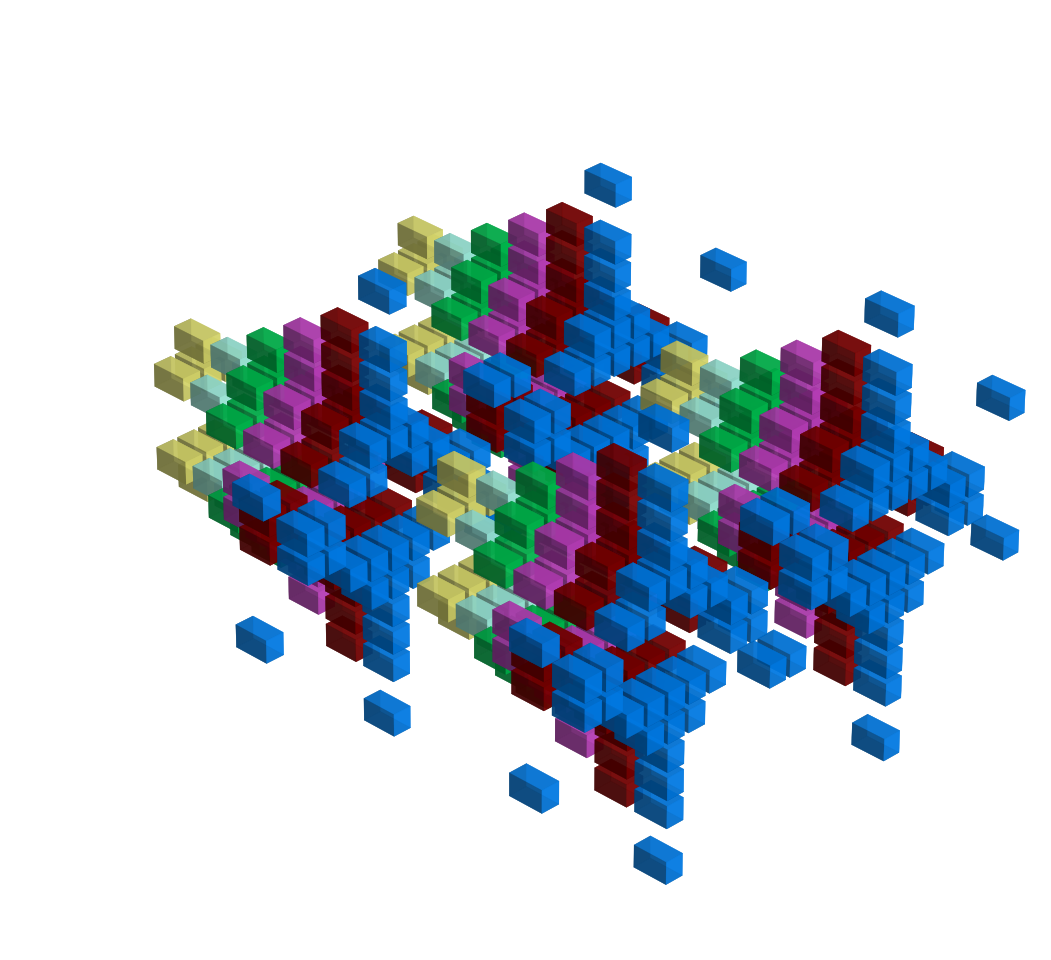
\includegraphics[width=5cm]{src/presets/pattern15-45.png}%           
  \end{adjustbox}                                                        
\caption{Preset 15.}                                           
\end{figure}                                                               

\clearpage
\begin{minipage}[b]{0.33\linewidth}
\begin{lrbox}{\mybox}%
\begin{lstlisting}[basicstyle=\ttfamily\tiny]
burstGeneratorF1
; currentSymmetrySetting
.BYTE  Y_AXIS_SYMMETRY
; smoothingDelay
.BYTE $0C
; Burst Position 1
.BYTE $07,$06
; Index to pattern 
.BYTE PULSAR
; Burst Position 2
.BYTE $11,$0D
; Index to pattern 
.BYTE PULSAR
; Burst Position 3
.BYTE $06,$11
; Index to pattern 
.BYTE PULSAR
; Burst Position 4
.BYTE $FF,$0B
; Index to pattern 
.BYTE PULSAR
; Burst Position 5
.BYTE $FF,$00
; Index to pattern 
.BYTE $FF
; Burst Position 6
.BYTE $21,$06
; Index to pattern 
.BYTE $00
; Burst Position 7
.BYTE $06,$01
; Index to pattern 
.BYTE $06
; Burst Position 8
.BYTE $41,$FF
; Index to pattern 
.BYTE $00
; Burst Position 9
.BYTE $06,$01
; Index to pattern 
.BYTE $06
; Burst Position 10
.BYTE $01,$06
; Index to pattern 
.BYTE $00

burstGeneratorF2
; currentSymmetrySetting
.BYTE Y_AXIS_SYMMETRY
; smoothingDelay
.BYTE $0C
; Burst Position 1
.BYTE $13,$08
; Index to pattern 
.BYTE STARONE
; Burst Position 2
.BYTE $07,$0F
; Index to pattern 
.BYTE STARONE
; Burst Position 3
.BYTE $FF,$00
; Index to pattern 
.BYTE MULTICROSS
; Burst Position 4
.BYTE $01,$2A
; Index to pattern 
.BYTE $41
; Burst Position 5
.BYTE $02,$00
; Index to pattern 
.BYTE $04
; Burst Position 6
.BYTE $62,$FF
; Index to pattern 
.BYTE $41
; Burst Position 7
.BYTE $06,$40
; Index to pattern 
.BYTE $00
; Burst Position 8
.BYTE $6B,$04
; Index to pattern 
.BYTE $41
; Burst Position 9
.BYTE $FF,$00
; Index to pattern 
.BYTE $FF
; Burst Position 10
.BYTE $00,$FF
; Index to pattern 
.BYTE $00
\end{lstlisting}
\end{lrbox}%
\scalebox{0.8}{\usebox{\mybox}}
\end{minipage}
\begin{minipage}[b]{0.33\linewidth}
\begin{lrbox}{\mybox}%
\begin{lstlisting}[basicstyle=\ttfamily\tiny]
burstGeneratorF3
; currentSymmetrySetting
.BYTE QUAD_SYMMETRY
; smoothingDelay
.BYTE $01
; Burst Position 1  
.BYTE $08,$01
; Index to pattern 
.BYTE LALLAMITA
; Burst Position 2
.BYTE $FF,$01
; Index to pattern 
.BYTE LALLAMITA
; Burst Position 3
.BYTE $08,$01
; Index to pattern 
.BYTE $02
; Burst Position 4
.BYTE $08,$01
; Index to pattern 
.BYTE $02
; Burst Position 5
.BYTE $08,$01
; Index to pattern 
.BYTE $02
; Burst Position 6
.BYTE $08,$01
; Index to pattern 
.BYTE $02
; Burst Position 7
.BYTE $08,$01
; Index to pattern 
.BYTE $02
; Burst Position 8
.BYTE $FF,$03
; Index to pattern 
.BYTE $02
; Burst Position 9
.BYTE $08,$03
; Index to pattern 
.BYTE $02
; Burst Position 10
.BYTE $08,$03
; Index to pattern 
.BYTE $02

burstGeneratorF4
; currentSymmetrySetting
.BYTE NO_SYMMETRY
; smoothingDelay:
.BYTE $11
; Burst Position 1
.BYTE $12,$09
; Index to pattern 
.BYTE CUSTOMPATTERN0
; Burst Position 2
.BYTE $FF,$08
; Index to pattern 
.BYTE STARTWO
; Burst Position 3
.BYTE $02,$08
; Index to pattern 
.BYTE $03
; Burst Position 4
.BYTE $02,$08
; Index to pattern 
.BYTE $03
; Burst Position 5
.BYTE $02,$FF
; Index to pattern 
.BYTE $00
; Burst Position 6
.BYTE $00,$00
; Index to pattern 
.BYTE $00
; Burst Position 7
.BYTE $01,$24
; Index to pattern 
.BYTE $00
; Burst Position 8
.BYTE $05,$01
; Index to pattern 
.BYTE $00
; Burst Position 9 
.BYTE $00,$00
; Index to pattern 
.BYTE $00
; Burst Position 10 
.BYTE $00,$BD
; Index to pattern 
.BYTE $00
\end{lstlisting}
\end{lrbox}%
\scalebox{0.8}{\usebox{\mybox}}
\end{minipage}
\begin{minipage}[b]{0.33\linewidth}
\begin{lrbox}{\mybox}%
\begin{lstlisting}[basicstyle=\ttfamily\tiny]
;--------------------
; Unused Data
;--------------------
.BYTE $00,$BD,$00,$B9,$00,$BD,$00,$BD
.BYTE $81,$BD,$81,$FF,$00,$BD,$F1,$FF
.BYTE $00,$28,$81,$FF,$81,$AE,$83,$AE
.BYTE $00,$FF,$81,$EE,$81,$AC,$C1,$BD
.BYTE $C1,$24,$81,$FF,$C1,$FF,$00,$EE
.BYTE $81,$BF,$85,$AE,$81,$EC,$E1,$BF
.BYTE $83,$37,$00,$EE,$81,$BF,$C3,$2E
.BYTE $81,$2E,$00,$FF,$00,$FF,$00,$FD
.BYTE $05,$DC,$02,$EE,$81,$EC,$C7,$0C
.BYTE $00,$68,$81,$EC,$03,$EE,$81,$EE
.BYTE $85,$62,$81,$EE,$01,$EC,$87,$EA
.BYTE $85,$FD,$83,$CD,$42,$EF,$00,$FF
.BYTE $00,$28,$02,$EA,$81,$BD,$85,$BF
.BYTE $81,$FF,$85,$EE,$00,$BF,$87,$BF
.BYTE $00,$EE,$87,$FF,$81,$FF,$A7,$FE
.BYTE $01,$FF,$80,$EE,$FD,$FF,$FF,$FF
\end{lstlisting}
\end{lrbox}%
\scalebox{0.8}{\usebox{\mybox}}
\end{minipage}
\clearpage
\rhead[]{Bursts}
\textbf{Lines 2800-3200.} This is the data used for generating 'bursts', the subject of our chapter
\hyperref[sec:bursts]{\textcolor{blue}{'beatific bursts'}}. 

Only four are defined, each bound to one of the 'Function' keys on the C64 keyboard. Each burst consists of
a header specifying the symmetry and smoothing delay used for the burst:
\begin{lstlisting}
; currentSymmetrySetting
.BYTE NO_SYMMETRY
; smoothingDelay:
.BYTE $11
\end{lstlisting}

.. followed by a sequence of 'cells' of three bytes each. Each cell gives the X and Y co-ordinates to place a pattern
and a reference to the pattern to draw:
\begin{lstlisting}
; Burst Position 1
.BYTE $12,$09
; Index to pattern 
.BYTE CUSTOMPATTERN0
\end{lstlisting}
\vfill
\begin{figure}[H]
    \centering
    \begin{adjustbox}{width=9cm,center}
      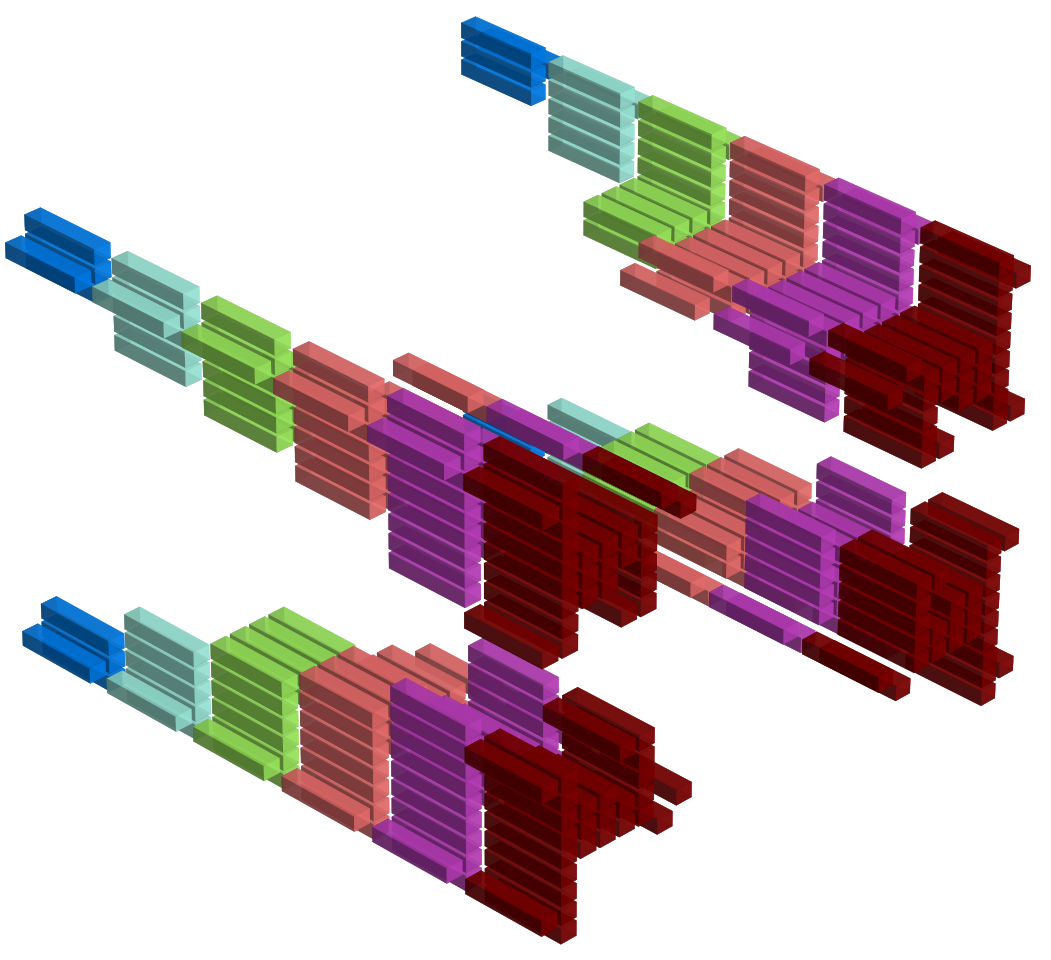
\includegraphics[width=1cm]{src/listing_commentary/diagrams/pattern1-0-45.png}%
      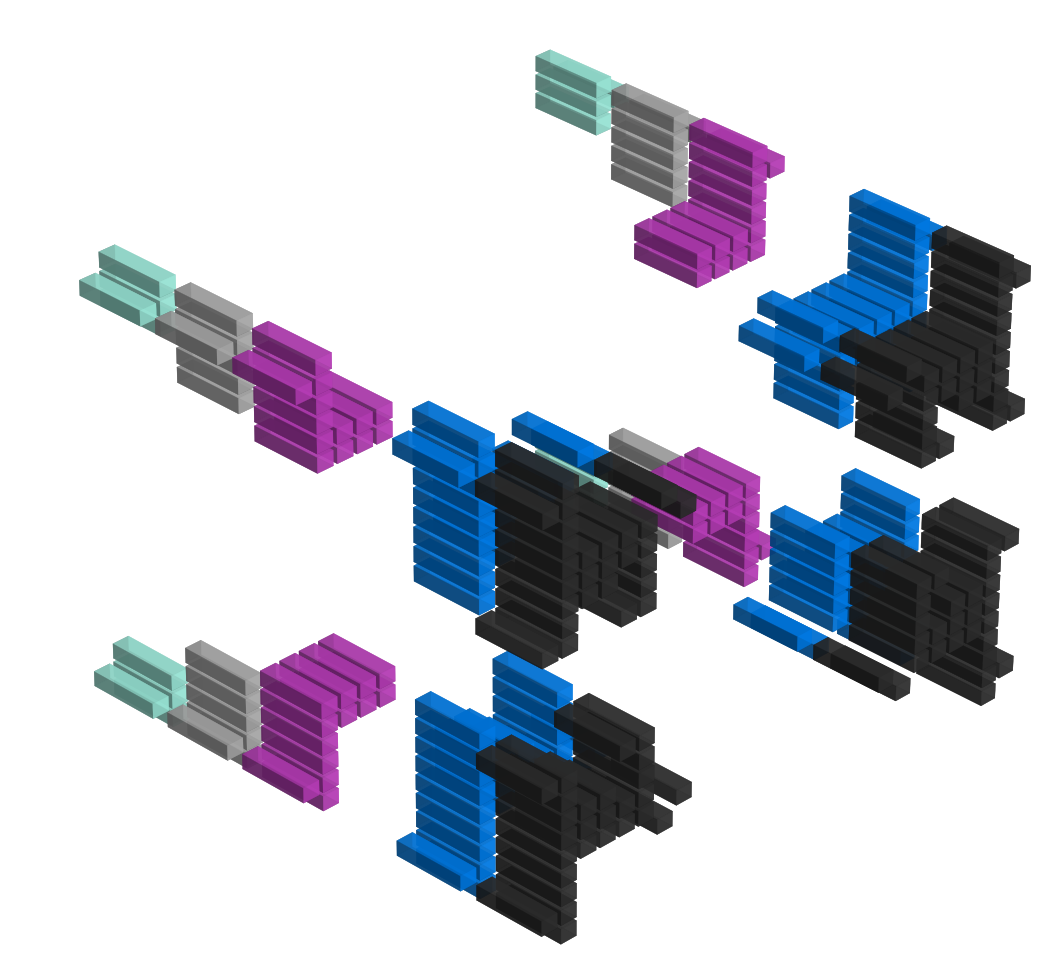
\includegraphics[width=1cm]{src/listing_commentary/diagrams/pattern1-1-45.png}%
    \end{adjustbox}
    \begin{adjustbox}{width=9cm,center}
      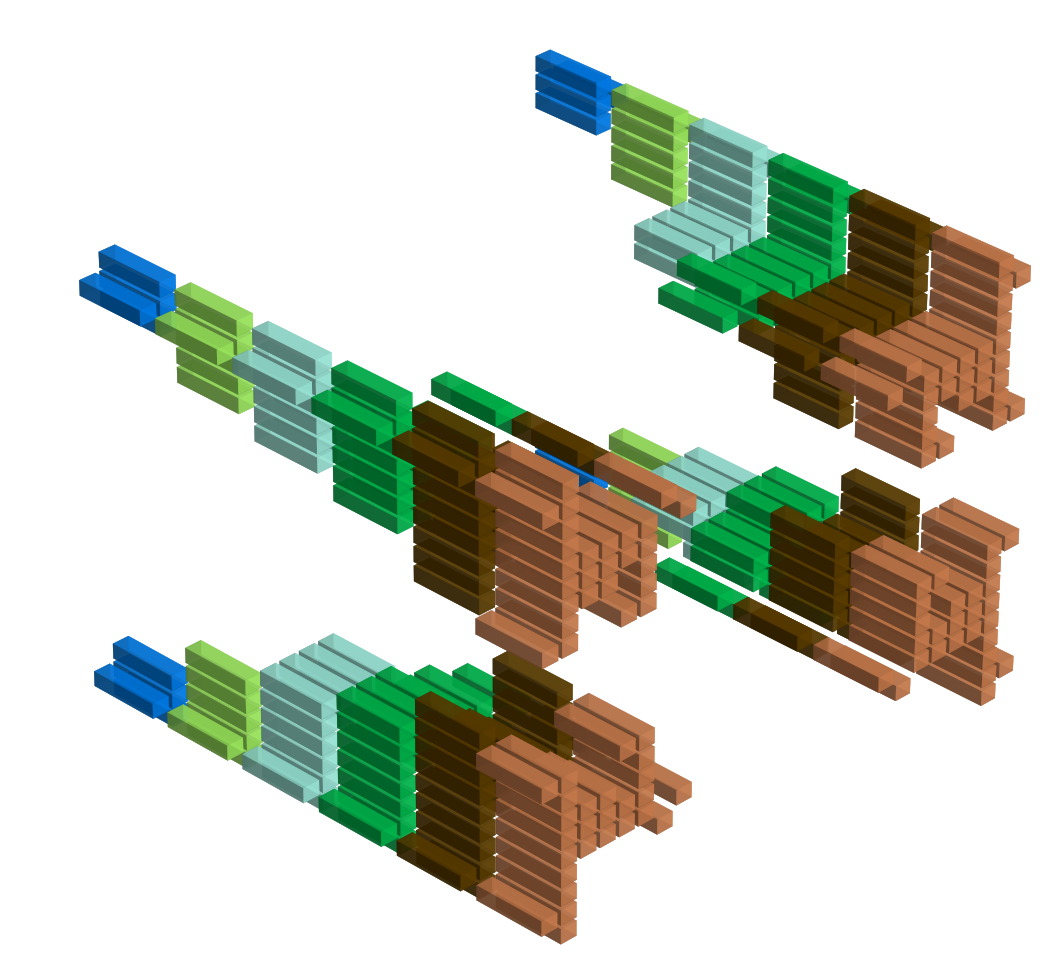
\includegraphics[width=1cm]{src/listing_commentary/diagrams/pattern1-2-45.png}%
      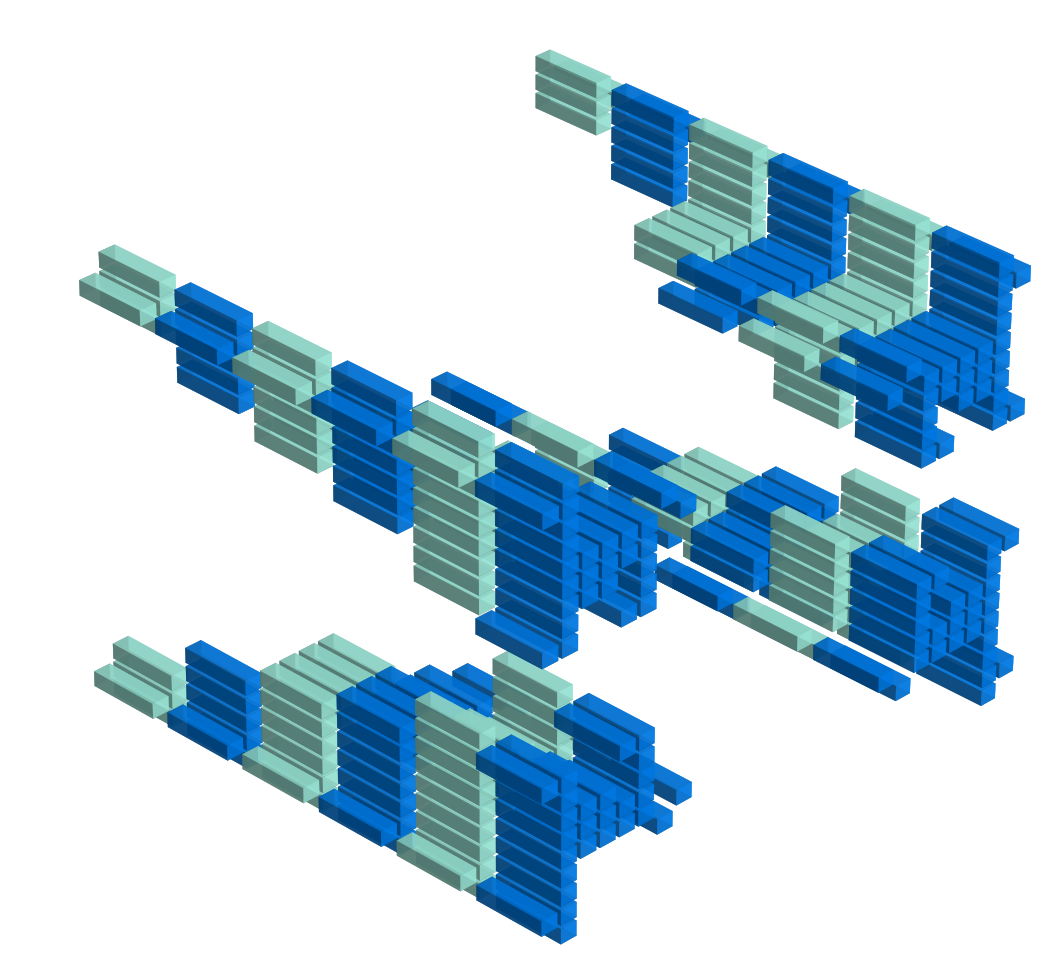
\includegraphics[width=1cm]{src/listing_commentary/diagrams/pattern1-3-45.png}%
    \end{adjustbox}
    \caption{The 'F2' burst in different color schemes}
\end{figure}

\clearpage
\begin{minipage}[b]{0.33\linewidth}
\begin{lrbox}{\mybox}%
\begin{lstlisting}[basicstyle=\ttfamily\tiny]
;-----------------------------------
; Sequencer Data
;-----------------------------------
startOfSequencerData = $C300
; currentSymmetrySetting
.BYTE $01
; smoothingDelay
.BYTE $0B
; Sequencer Position 1
.BYTE $04,$04  ; X/Y Co-ordinates
.BYTE PULSAR     ; Index to pattern    
; Sequencer Position 2
.BYTE $08,$09  ; X/Y Co-ordinates
.BYTE PULSAR   ; Index to pattern in patternIndexArray   
; Sequencer Position 3
.BYTE $0C,$0C  ; X/Y Co-ordinates
.BYTE PULSAR   ; Index to pattern
; Sequencer Position 4
.BYTE $10,$11  ; X/Y Co-ordinates
.BYTE PULSAR   ; Index to pattern
; Sequencer Position 5
.BYTE $14,$13  ; X/Y Co-ordinates
.BYTE PULSAR   ; Index to pattern
; Sequencer Position 6
.BYTE $17,$13  ; X/Y Co-ordinates
.BYTE PULSAR   ; Index to pattern
; Each triplet of bytes below
; follows the above pattern.
; The '$FF' below indicates the end of the
; sequencer data.
.BYTE $FF
.BYTE $01,$06,$41,$FF,$00,$06,$01,$06
.BYTE $01,$06,$00,$00,$FF,$06,$00,$02
.BYTE $00,$FF,$41,$46,$00,$06,$81,$AA
.BYTE $41,$02,$00,$04,$62,$FF,$41,$06
.BYTE $40,$00,$6B,$04,$C1,$FF,$00,$FF
.BYTE $00,$FF,$00,$42,$02,$AE,$01,$00
.BYTE $07,$1C,$80,$FF,$05,$06,$01,$02
.BYTE $07,$02,$05,$00,$85,$06,$01,$02
.BYTE $05,$02,$41,$00,$00,$06,$03,$BD
.BYTE $00,$BF,$00,$BF,$C5,$BF,$01,$00
.BYTE $42,$02,$40,$00,$40,$06,$01,$FF
.BYTE $00,$02,$40,$FF,$05,$02,$00,$00
.BYTE $00,$00,$01,$20,$00,$8D,$01,$00
.BYTE $00,$00,$00,$00,$BD,$00,$BD,$00
.BYTE $BD,$40,$BD,$81,$BD,$81,$FF,$00
.BYTE $FF,$F1,$FF,$00,$20,$81,$FF,$81
.BYTE $AE,$C3,$EE,$00,$FF,$81,$EE,$81
.BYTE $AC,$C1,$FD,$D1,$24,$81,$FF,$C1
.BYTE $FF,$00,$AE,$81,$FF,$C5,$EE,$41
.BYTE $EC,$E1,$FF,$C3,$37,$00,$EE,$C1
.BYTE $BF,$C3,$AE,$C1,$AE,$00,$FF,$00
.BYTE $FF,$00,$FD,$05,$DD,$03,$EE,$85
.BYTE $EC,$C7,$4C,$00,$60,$81,$EC,$87
.BYTE $EE,$81,$EE,$8D,$62,$85,$EE,$85
.BYTE $EE,$87,$EA,$85,$FD,$83,$ED,$42
.BYTE $EF,$00,$FF,$40,$28,$02,$EE,$C1
.BYTE $BD,$85,$FF,$81,$FF,$85,$EE,$00
.BYTE $FF,$A7,$BF,$00,$EE,$87,$FF,$81
.BYTE $FF,$A7,$FE,$01,$FF,$00,$EE,$FD
.BYTE $FF,$FF,$FF,$FF,$00,$F7,$00,$FF
.BYTE $00,$BF,$40,$46,$00,$06,$00,$FF
.BYTE $00,$06,$00,$FF,$01,$06,$00,$06
.BYTE $01,$06,$41,$FF,$00,$06,$01,$06
.BYTE $01,$06,$00,$00,$FF,$06,$00,$02
.BYTE $00,$FF,$41,$46,$00,$06,$01,$2A
.BYTE $41,$02,$00,$04,$6A,$FF,$41,$06
.BYTE $40,$00,$4B,$04,$89,$FF,$00,$FF
.BYTE $00,$FF,$00,$42,$02,$BF,$01,$00
.BYTE $07,$1C,$00,$FF,$05,$06,$01,$02
.BYTE $07,$02,$05,$00,$05,$06,$01,$02
.BYTE $05,$02,$01,$00,$00,$06,$02,$BD
.BYTE $00,$BF,$00,$FF,$C5,$BF,$01,$00
.BYTE $42,$02,$40,$00,$40,$06,$01,$FF
.BYTE $00,$02,$40,$FF,$45,$02,$00,$00
.BYTE $00,$02,$01,$24,$00,$05,$01,$00
.BYTE $00,$00,$00,$00,$BD,$00,$B9,$00
.BYTE $BD,$40,$BD,$81,$BD,$81,$FF,$00
.BYTE $FD,$F1,$FF,$00,$20,$81,$FF,$C1
.BYTE $AE,$83,$EE,$00,$FF,$81,$EE,$81
.BYTE $AC,$C1,$BD,$C1,$24,$C1,$FF,$C1
.BYTE $FF,$00,$EE,$81,$FD,$C5,$EE,$C1
.BYTE $EC,$E1,$FF,$C3,$37,$00,$EE,$C1
.BYTE $BF,$C3,$AE,$C1,$AE,$00,$FF,$00
.BYTE $FF,$00,$FD,$81,$DD,$03,$EA,$81
.BYTE $EC,$C7,$CC,$00,$60,$81,$EC,$83
.BYTE $EE,$81,$EE,$85,$62,$81,$EE,$81
.BYTE $EE,$87,$EA,$85,$FD,$83,$ED,$42
.BYTE $EF,$00,$FF,$00,$28,$02,$EE,$81
.BYTE $FD,$85,$FF,$81,$FF,$85,$EE,$00
.BYTE $FD,$85,$FF,$00,$EE,$87,$FF,$81
.BYTE $FF,$A7,$FF,$01,$FF,$80,$EE,$FD
.BYTE $FF,$FF,$FF,$FF,$00,$F7,$00,$FF
.BYTE $00,$BF,$40,$06,$00,$06,$00,$FF
\end{lstlisting}
\end{lrbox}%
\scalebox{0.8}{\usebox{\mybox}}
\end{minipage}
\begin{minipage}[b]{0.33\linewidth}
\begin{lrbox}{\mybox}%
\begin{lstlisting}[basicstyle=\ttfamily\tiny]
.BYTE $00,$06,$00,$FF,$21,$06,$00,$06
.BYTE $01,$06,$01,$BF,$00,$06,$01,$06
.BYTE $01,$06,$00,$00,$FF,$06,$00,$02
.BYTE $00,$FF,$41,$46,$00,$06,$01,$2A
.BYTE $01,$02,$00,$04,$62,$FF,$01,$06
.BYTE $40,$00,$6B,$04,$91,$BF,$00,$FF
.BYTE $00,$FF,$00,$42,$02,$BF,$01,$00
.BYTE $07,$1C,$80,$FF,$25,$06,$01,$02
.BYTE $07,$02,$05,$00,$85,$06,$01,$02
.BYTE $05,$02,$01,$00,$00,$06,$03,$BD
.BYTE $00,$BF,$00,$BF,$C5,$BF,$01,$00
.BYTE $42,$02,$40,$00,$00,$06,$01,$FF
.BYTE $00,$02,$40,$FF,$05,$02,$00,$00
.BYTE $00,$00,$01,$20,$00,$8D,$01,$00
.BYTE $00,$00,$00,$00,$BD,$00,$B9,$00
.BYTE $BD,$40,$BD,$81,$BD,$81,$FF,$00
.BYTE $BF,$F9,$FF,$00,$28,$81,$FF,$81
.BYTE $AE,$83,$AE,$00,$FF,$81,$EE,$81
.BYTE $AC,$C1,$BD,$A1,$24,$C1,$FF,$C1
.BYTE $FF,$00,$AE,$81,$BF,$C5,$EE,$C1
.BYTE $EC,$E1,$BF,$83,$3F,$00,$EE,$C1
.BYTE $BF,$E3,$AE,$C1,$AE,$20,$FF,$00
.BYTE $FF,$00,$BD,$05,$DD,$03,$EA,$81
.BYTE $EC,$C7,$4C,$00,$68,$81,$EC,$87
.BYTE $EE,$81,$EE,$AD,$62,$85,$EE,$81
.BYTE $EE,$87,$EA,$85,$FD,$83,$EC,$42
.BYTE $EF,$00,$FF,$00,$28,$02,$EE,$81
.BYTE $BD,$A5,$BF,$81,$BF,$85,$EE,$00
.BYTE $BF,$AF,$BF,$00,$EC,$87,$FF,$81
.BYTE $FF,$A7,$EE,$01,$FF,$80,$EE,$FD
.BYTE $FF,$FF
.BYTE $FF,$FF,$00,$F7,$00,$FF,$00,$BF
.BYTE $40,$46,$00,$06,$00,$FF,$00,$06
.BYTE $00,$FF,$A1,$06,$00,$06,$01,$06
.BYTE $41,$FF,$00,$06,$01,$06,$01,$06
.BYTE $00,$00,$FF,$06,$00,$02,$00,$FF
.BYTE $41,$46,$00,$06,$81,$2A,$01,$02
.BYTE $00,$04,$62,$FF,$41,$06,$40,$00
.BYTE $6B,$04,$B1,$FB,$00,$FF,$00,$FF
.BYTE $00,$42,$02,$B6,$01,$00,$07,$1C
.BYTE $80,$FF,$25,$06,$01,$02,$07,$02
.BYTE $05,$00,$85,$06,$01,$02,$05,$02
.BYTE $01,$00,$00,$06,$03,$BD,$00,$BF
.BYTE $00,$BF,$C5,$BF,$01,$00,$42,$02
.BYTE $40,$00,$40,$06,$01,$FF,$00,$02
.BYTE $40,$FF,$45,$02,$00,$02,$00,$00
.BYTE $01,$A0,$00,$8F,$01,$00,$00,$00
.BYTE $00,$00,$BD,$00,$BD,$00,$BD,$40
.BYTE $BD,$81,$BD,$81,$FF,$00,$FD,$F1
.BYTE $FF,$00,$20,$81,$FF,$81,$AC,$83
.BYTE $EE,$00,$FF,$81,$EE,$81,$AC,$C1
.BYTE $BD,$C1,$24,$C1,$FF,$C1,$FF,$00
.BYTE $EE,$81,$FD,$C5,$AE,$C1,$EC,$E1
.BYTE $BF,$C3,$3F,$00,$EE,$C1,$BF,$C3
.BYTE $AE,$C1,$EE,$00,$FF,$00,$FF,$00
.BYTE $FD,$85,$DD,$03,$EE,$85,$EC,$C7
.BYTE $CC,$00,$E8,$81,$EC,$87,$EE,$81
.BYTE $EE,$8D,$62,$81,$EE,$81,$EE,$87
.BYTE $EA,$85,$FD,$83,$CC,$42,$EF,$00
.BYTE $FF,$00,$28,$02,$EE,$C1,$FD,$85
.BYTE $FF,$81,$FF,$85,$EE,$00,$FD,$85
.BYTE $BF,$00,$EE,$87,$FF,$81,$FF,$87
.BYTE $FE,$01,$FF,$80,$EE,$FD,$FF,$FF
.BYTE $FF,$FF,$00,$F7,$00,$FF,$00,$BF
.BYTE $40,$46,$00,$06,$00,$FF,$00,$06
.BYTE $00,$FF,$11,$06,$00,$06,$01,$06
.BYTE $41,$FF,$00,$06,$01,$06,$01,$06
.BYTE $00,$00,$FF,$06,$00,$02,$00,$FF
.BYTE $41,$46,$00,$06,$01,$AB,$41,$02
.BYTE $00,$04,$62,$FF,$41,$06,$40,$00
.BYTE $6B,$04,$91,$FF,$00,$FF,$00,$FF
.BYTE $00,$42,$02,$27,$01,$00,$07,$1C
.BYTE $00,$FF,$25,$06,$05,$02,$07,$02
.BYTE $05,$00,$05,$06,$01,$02,$05,$02
.BYTE $41,$00,$00,$06,$03,$BD,$00,$BF
.BYTE $00,$BD,$C5,$BF,$01,$00,$42,$02
.BYTE $41,$00,$40,$06,$01,$FF,$00,$02
.BYTE $41,$FF,$45,$02,$00,$00,$00,$00
.BYTE $01,$24,$00,$0D,$01,$00,$00,$00
.BYTE $00,$00,$BD,$00,$FD,$00,$FD,$40
.BYTE $BD,$81,$BD,$81,$FF,$00,$FF,$F1
.BYTE $FF,$00,$20,$81,$FF,$81,$AE,$C3
.BYTE $EE,$00,$FF,$81,$EE,$81,$AC,$C1
.BYTE $FD,$81,$24,$C1,$FF,$C1,$FF,$00
.BYTE $EE,$81,$FF,$C5,$EE,$41,$EC,$E1
.BYTE $FF,$C3,$37,$00,$EE,$C1,$BF,$C3
.BYTE $A6,$C1,$A6,$00,$FF,$00,$FF,$00
.BYTE $BF,$05,$FD,$03,$EA,$85,$EC,$C7
.BYTE $DD,$00,$60,$81,$EC,$87,$EE,$81
.BYTE $EE,$85,$62,$81,$EE,$81,$EE,$87
.BYTE $EA,$85,$FD,$83,$EC,$40,$EF,$00
.BYTE $FF,$00,$28,$02,$EA,$C1,$AC,$85
.BYTE $BF,$81,$FF,$85,$EE,$00,$FF,$C7
.BYTE $BF,$00,$EE,$87,$FF,$81,$FF,$87
.BYTE $FE,$01,$FF,$00,$EE,$FD,$FF,$FF
.BYTE $FF

\end{lstlisting}
\end{lrbox}%
\scalebox{0.8}{\usebox{\mybox}}
\end{minipage}
\clearpage
\rhead[]{Sequencer}
\textbf{Lines 2300-2800.} This data supports Psychedelia's sequencer which we cover in 
\hyperref[sec:sequencer]{\textcolor{blue}{'sensitive sequencer'}}.  Like the burst data it consists of a header, again defining the symmetry and smoothing delay:
\begin{lstlisting}
; currentSymmetrySetting
.BYTE $01
; smoothingDelay
.BYTE $0B
\end{lstlisting}

Again like the burst data, the rest of the data consists of cells of three bytes defining X and Y co-ordinates
and a pattern:
\begin{lstlisting}
; Sequencer Position 1
.BYTE $04,$04  ; X/Y Co-ordinates
.BYTE PULSAR     ; Index to pattern    
\end{lstlisting}
\vfill
\begin{figure}[H]
    \centering
    \begin{adjustbox}{width=10cm,center}
      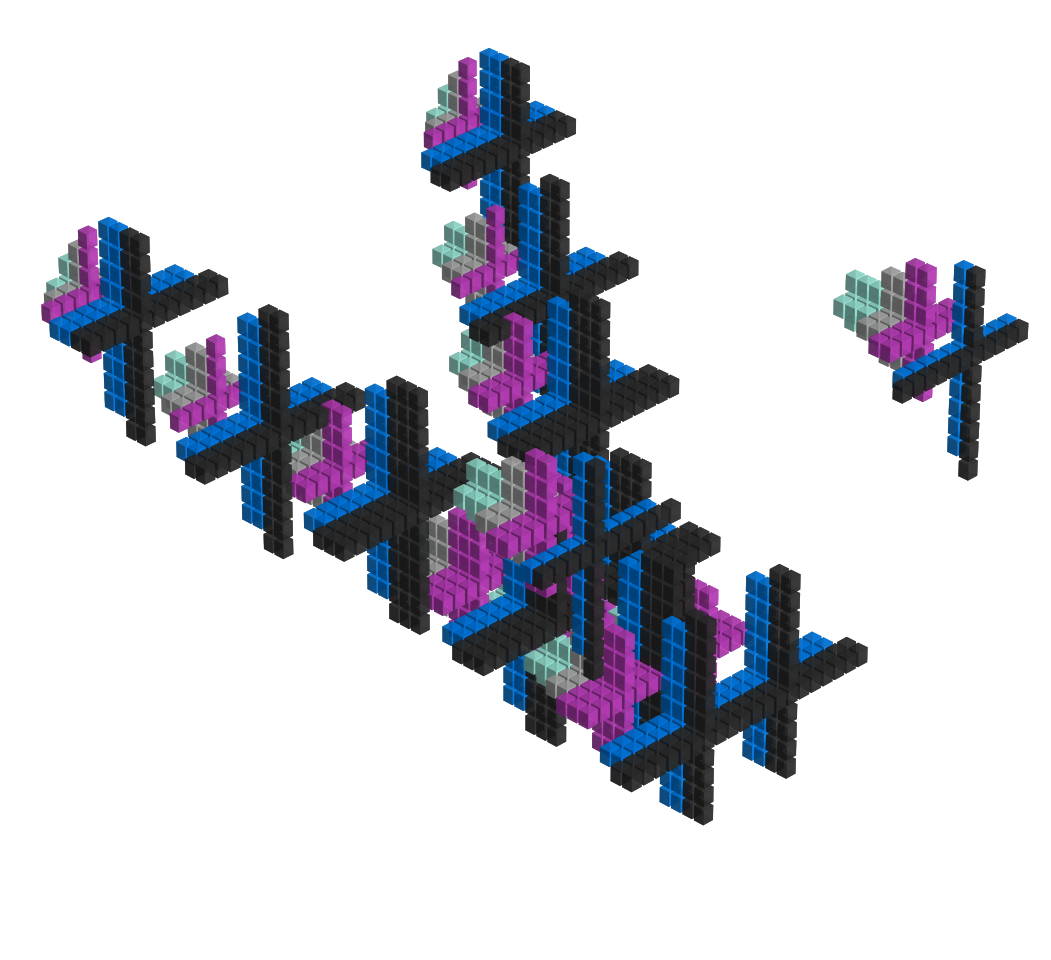
\includegraphics[width=2cm]{src/listing_commentary/sequencer/pattern1-0-45.png}%
      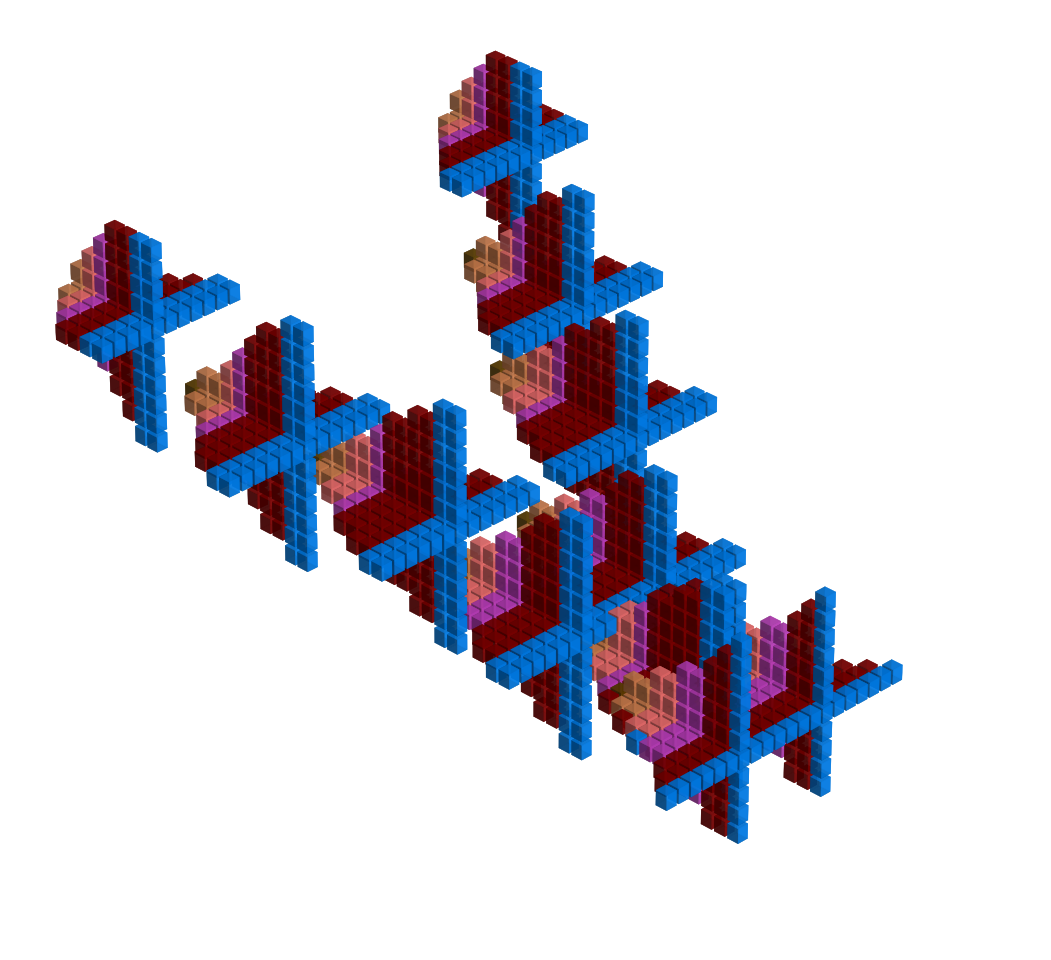
\includegraphics[width=2cm]{src/listing_commentary/sequencer/pattern1-1-45.png}%
    \end{adjustbox}
    \begin{adjustbox}{width=10cm,center}
      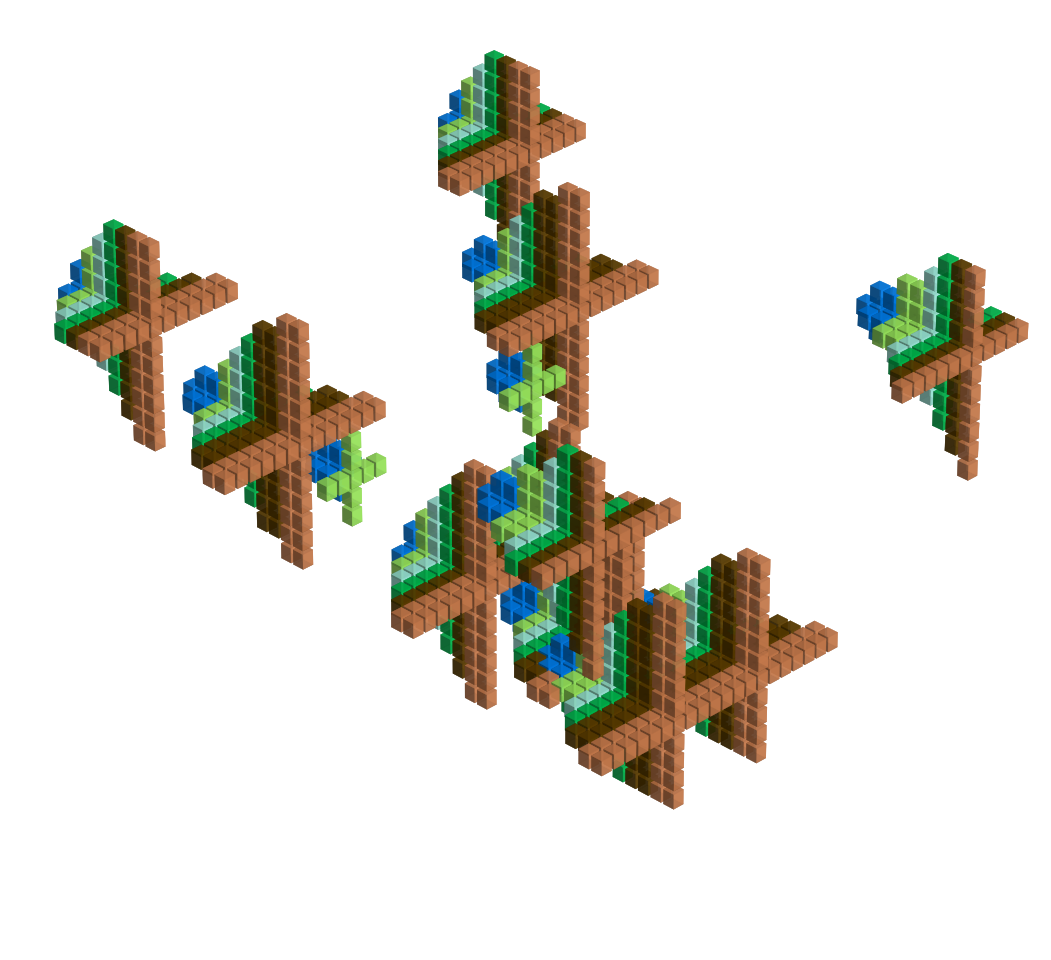
\includegraphics[width=2cm]{src/listing_commentary/sequencer/pattern1-3-45.png}%
      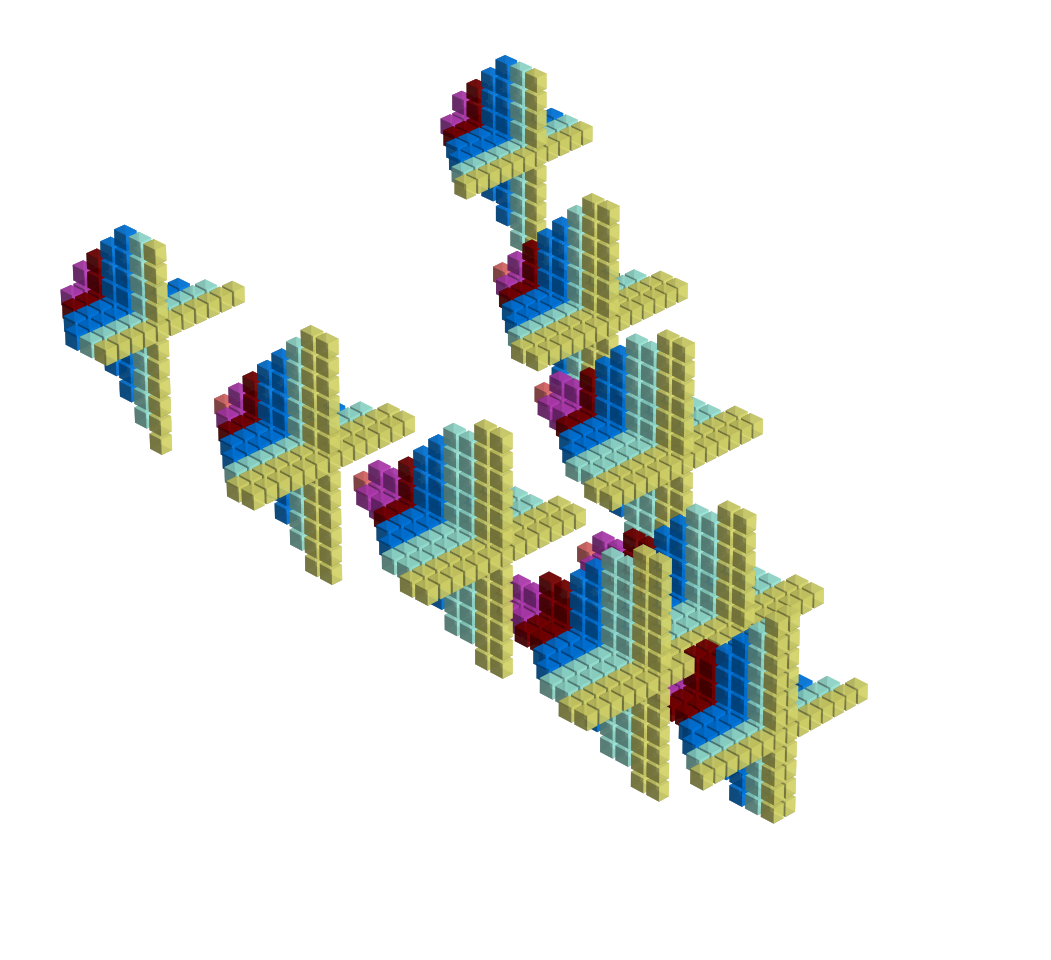
\includegraphics[width=2cm]{src/listing_commentary/sequencer/pattern1-4-45.png}%
    \end{adjustbox}
    \caption{The sequencer in different color schemes}
\end{figure}

\clearpage
\rhead[]{Custom Patterns}
\begin{minipage}[b]{0.33\linewidth}
\begin{lrbox}{\mybox}%
\begin{lstlisting}[basicstyle=\ttfamily\tiny]
;
;    33033   
;  35  0  54 
; 5    6    5
; 3   020   4
;    0 2 0   
;  30  2  14 
;    54245   
;
customPattern0XPosArray
.BYTE $00,$00,$00,$FF,$FE,$FD,$01,$02,$55
.BYTE $00,$03,$55
.BYTE $00,$00,$00,$00,$00,$55
.BYTE $00,$FF,$FE,$FC,$FB,$FC,$01,$02,$55
.BYTE $00,$04,$05,$04,$FF,$01,$55
.BYTE $00,$FD,$FB,$03,$05,$02,$FE,$55
.BYTE $00,$55

.BYTE $00,$00,$00,$00
.BYTE $00,$00,$00,$00,$00,$00,$00,$00
.BYTE $00,$00,$00,$00,$00,$00,$00,$00
.BYTE $00,$00,$00,$00,$00,$00,$00,$00
.BYTE $00,$00,$00,$00,$00,$00,$00,$00
.BYTE $00,$00,$00,$00,$00,$00,$00,$00
.BYTE $00,$00,$00,$00,$00,$00,$00,$00
.BYTE $00,$00,$00,$00,$00,$00,$00,$00
.BYTE $00,$00,$00,$00,$00,$00,$00,$00
.BYTE $00,$00,$00,$00,$00,$00,$00,$00
.BYTE $00,$00,$00,$00,$00,$00,$00,$00

; customPattern0YPosArray
.BYTE $00,$FF,$FE,$01,$02,$03,$01,$02,$55
.BYTE $00,$03,$55
.BYTE $00,$01,$02,$03,$04,$55
.BYTE $00,$FE,$FE,$FF,$01,$03,$FE,$FE,$55
.BYTE $00,$FF,$01,$03,$04,$04,$55
.BYTE $00,$FF,$00,$FF,$00,$04,$04,$55
.BYTE $00,$55

.BYTE $00,$00,$00,$00
.BYTE $00,$00,$00,$00,$00,$00,$00,$00
.BYTE $00,$00,$00,$00,$00,$00,$00,$00
.BYTE $00,$00,$00,$00,$00,$00,$00,$00
.BYTE $00,$00,$00,$00,$00,$00,$00,$00
.BYTE $00,$00,$00,$00,$00,$00,$00,$00
.BYTE $00,$00,$00,$00,$00,$00,$00,$00
.BYTE $00,$00,$00,$00,$00,$00,$00,$00
.BYTE $00,$00,$00,$00,$00,$00,$00,$00
.BYTE $00,$00,$00,$00,$00,$00,$00,$00
.BYTE $00,$00,$00,$00,$00,$00,$00,$00
;       3      
;    4  5  4   
;       6      
; 3     1     3
;       7      
;     21 12    
;  466     664 
;              
;              
;    3  5  3   
;-----------------
; customPattern1XPosArray
.BYTE $00,$00,$FF,$01,$55
.BYTE $00,$FE,$02,$55
.BYTE $00,$00,$FA,$06,$03,$FD,$55
.BYTE $00,$FD,$03,$FB,$05,$55
.BYTE $00,$00,$00,$55
.BYTE $00,$00,$FC,$04,$03,$FD,$55
.BYTE $00,$55

.BYTE $00,$00,$00,$00,$00
.BYTE $00,$00,$00,$00,$00,$00,$00,$00
.BYTE $00,$00,$00,$00,$00,$00,$00,$00
.BYTE $00,$00,$00,$00,$00,$00,$00,$00
.BYTE $00,$00,$00,$00,$00,$00,$00,$00
.BYTE $00,$00,$00,$00,$00,$00,$00,$00
.BYTE $00,$00,$00,$00,$00,$00,$00,$00
.BYTE $00,$00,$00,$00,$00,$00,$00,$00
.BYTE $00,$00,$00,$00,$00,$00,$00,$00
.BYTE $00,$00,$00,$00,$00,$00,$00,$00
.BYTE $00,$00,$00,$00,$00,$00,$00,$00
.BYTE $00,$00,$00,$00,$00,$00,$00,$00

; customPattern1YPosArray
.BYTE $00,$FF,$01,$01,$55
.BYTE $00,$01,$01,$55
.BYTE $00,$FC,$FF,$FF,$05,$05,$55
.BYTE $00,$FD,$FD,$02,$02,$55
.BYTE $00,$05,$FD,$55
.BYTE $00,$FE,$02,$02,$02,$02,$55
.BYTE $00,$55

.BYTE $00,$00,$00,$00,$00
.BYTE $00,$00,$00,$00,$00,$00,$00,$00
.BYTE $00,$00,$00,$00,$00,$00,$00,$00
.BYTE $00,$00,$00,$00,$00,$00,$00,$00
.BYTE $00,$00,$00,$00,$00,$00,$00,$00
.BYTE $00,$00,$00,$00,$00,$00,$00,$00
.BYTE $00,$00,$00,$00,$00,$00,$00,$00
.BYTE $00,$00,$00,$00,$00,$00,$00,$00
.BYTE $00,$00,$00,$00,$00,$00,$00,$00
.BYTE $00,$00,$00,$00,$00,$00,$00,$00
.BYTE $00,$00,$00,$00,$00,$00,$00,$00
.BYTE $00,$00,$00,$00,$00,$00,$00,$00

\end{lstlisting}
\end{lrbox}%
\scalebox{0.8}{\usebox{\mybox}}
\end{minipage}
\begin{minipage}[b]{0.33\linewidth}
\begin{lrbox}{\mybox}%
\begin{lstlisting}[basicstyle=\ttfamily\tiny]

;        5       
;      8   8     
;   4         4  
;                
;                
; 3   2  9  2   3
;                
;                
;        6       
;-----------------
customPattern2XPosArray
.BYTE $00,$55
.BYTE $00,$FD,$03,$55
.BYTE $00,$F9,$07,$55
.BYTE $00,$FB,$05,$55
.BYTE $00,$00,$55
.BYTE $00,$00,$55
.BYTE $00,$55
.BYTE $FE,$02,$55
.BYTE $00,$55
.BYTE $55

.BYTE $00,$00,$00,$00
.BYTE $00,$00,$00,$00,$00,$00,$00,$00
.BYTE $00,$00,$00,$00,$00,$00,$00,$00
.BYTE $00,$00,$00,$00,$00,$00,$00,$00
.BYTE $00,$00,$00,$00,$00,$00,$00,$00
.BYTE $00,$00,$00,$00,$00,$00,$00,$00
.BYTE $00,$00,$00,$00,$00,$00,$00,$00
.BYTE $00,$00,$00,$00,$00,$00,$00,$00
.BYTE $00,$00,$00,$00,$00,$00,$00,$00
.BYTE $00,$00,$00,$00,$00,$00,$00,$00

; customPattern2YPosArray
.BYTE $00,$55
.BYTE $00,$00,$00,$55
.BYTE $00,$00,$00,$55
.BYTE $00,$FD,$FD,$55
.BYTE $00,$FB,$55
.BYTE $00,$04,$55
.BYTE $00,$55
.BYTE $FC,$FC,$55
.BYTE $00,$55
.BYTE $55
.BYTE $00,$00,$00,$00
.BYTE $00,$00,$00,$00,$00,$00,$00,$00
.BYTE $00,$00,$00,$00,$00,$00,$00,$00
.BYTE $00,$00,$00,$00,$00,$00,$00,$00
.BYTE $00,$00,$00,$00,$00,$00,$00,$00
.BYTE $00,$00,$00,$00,$00,$00,$00,$00
.BYTE $00,$00,$00,$00,$00,$00,$00,$00
.BYTE $00,$00,$00,$00,$00,$00,$00,$00
.BYTE $00,$00,$00,$00,$00,$00,$00,$00
.BYTE $00,$00,$00,$00,$00,$00,$00,$00
.BYTE $00,$00,$00,$00,$00,$00,$00,$00
.BYTE $00,$00,$00,$00,$00,$00,$00,$00

;  5    
; 66  1 
;  4 711
;   4222
;    3 2
;    3 3
;-----------------
; customPattern3XPosArray
.BYTE $00,$01,$01,$02,$55
.BYTE $00,$00,$01,$02,$02,$55
.BYTE $00,$00,$00,$02,$55
.BYTE $00,$FF,$FE,$55
.BYTE $00,$FE,$FE,$55
.BYTE $00,$FD,$FE,$55
.BYTE $00,$55

.BYTE $00,$00
.BYTE $00,$00,$00,$00,$00,$00,$00,$00
.BYTE $00,$00,$00,$00,$00,$00,$00,$00
.BYTE $00,$00,$00,$00,$00,$00,$00,$00
.BYTE $00,$00,$00,$00,$00,$00,$00,$00
.BYTE $00,$00,$00,$00,$00,$00,$00,$00
.BYTE $00,$00,$00,$00,$00,$00,$00,$00
.BYTE $00,$00,$00,$00,$00,$00,$00,$00
.BYTE $00,$00,$00,$00,$00,$00,$00,$00
.BYTE $00,$00,$00,$00,$00,$00,$00,$00
.BYTE $00,$00,$00,$00,$00,$00,$00,$00
.BYTE $00,$00,$00,$00,$00,$00,$00,$00

; customPattern3YPosArray
.BYTE $00,$FF,$00,$00,$55
.BYTE $00,$01,$01,$01,$02,$55
.BYTE $00,$02,$03,$03,$55
.BYTE $00,$01,$00,$55
.BYTE $00,$FF,$FE,$55
.BYTE $00,$FF,$FF,$55
.BYTE $00,$55

.BYTE $00,$00
.BYTE $00,$00,$00,$00,$00,$00,$00,$00
.BYTE $00,$00,$00,$00,$00,$00,$00,$00
.BYTE $00,$00,$00,$00,$00,$00,$00,$00
.BYTE $00,$00,$00,$00,$00,$00,$00,$00
.BYTE $00,$00,$00,$00,$00,$00,$00,$00
.BYTE $00,$00,$00,$00,$00,$00,$00,$00
.BYTE $00,$00,$00,$00,$00,$00,$00,$00
.BYTE $00,$00,$00,$00,$00,$00,$00,$00
.BYTE $00,$00,$00,$00,$00,$00,$00,$00
.BYTE $00,$00,$00,$00,$00,$00,$00,$00
.BYTE $00,$00,$00,$00,$00,$00,$00,$00
\end{lstlisting}
\end{lrbox}%
\scalebox{0.8}{\usebox{\mybox}}
\end{minipage}
\begin{minipage}[b]{0.33\linewidth}
\begin{lrbox}{\mybox}%
\begin{lstlisting}[basicstyle=\ttfamily\tiny]



;                1                    
;                                     
;                                     
;                                     
;                                     
;                3                    
;                                     
;                                     
;                4                    
;                                     
;                5                    
;                6                    
; 1    2     99 6106899      2    1
;                                     
;                                     
;                                     
;                                     
;                                     
;                                     
;                                     
;                                     
;                                     
;                                     
;                1                    
; customPattern4XPosArray
.BYTE $00,$00,$00,$ED,$14,$55
.BYTE $00,$F2,$0F,$55
.BYTE $00,$00,$55
.BYTE $00,$00,$55
.BYTE $00,$00,$55
.BYTE $00,$00,$FF,$01,$55
.BYTE $00,$55
.BYTE $02,$55
.BYTE $00,$FC,$FD,$03,$04,$55
.BYTE $00,$55

.BYTE $00,$00,$00,$00
.BYTE $00,$00,$00,$00,$00,$00,$00,$00
.BYTE $00,$00,$00,$00,$00,$00,$00,$00
.BYTE $00,$00,$00,$00,$00,$00,$00,$00
.BYTE $00,$00,$00,$00,$00,$00,$00,$00
.BYTE $00,$00,$00,$00,$00,$00,$00,$00
.BYTE $00,$00,$00,$00,$00,$00,$00,$00
.BYTE $00,$00,$00,$00,$00,$00,$00,$00
.BYTE $00,$00,$00,$00,$00,$00,$00,$00
.BYTE $00,$00,$00,$00,$00,$00,$00,$00
.BYTE $00,$00,$00,$00,$00,$00,$00,$00
.BYTE $00,$00,$00,$00,$00,$00,$00,$00

; customPattern4YPosArray
.BYTE $00,$0B,$F4,$00,$00,$55
.BYTE $00,$00,$00,$55
.BYTE $00,$F9,$55
.BYTE $00,$FC,$55
.BYTE $00,$FE,$55
.BYTE $00,$FF,$00,$00,$55
.BYTE $00,$55
.BYTE $00,$55
.BYTE $00,$00,$00,$00,$00,$55
.BYTE $00,$55

.BYTE $00,$00,$00,$00
.BYTE $00,$00,$00,$00,$00,$00,$00,$00
.BYTE $00,$00,$00,$00,$00,$00,$00,$00
.BYTE $00,$00,$00,$00,$00,$00,$00,$00
.BYTE $00,$00,$00,$00,$00,$00,$00,$00
.BYTE $00,$00,$00,$00,$00,$00,$00,$00
.BYTE $00,$00,$00,$00,$00,$00,$00,$00
.BYTE $00,$00,$00,$00,$00,$00,$00,$00
.BYTE $00,$00,$00,$00,$00,$00,$00,$00
.BYTE $00,$00,$00,$00,$00,$00,$00,$00
.BYTE $00,$00,$00,$00,$00,$00,$00,$00
.BYTE $00,$00,$00,$00,$00,$00,$00,$00






























;
\end{lstlisting}
\end{lrbox}%
\scalebox{0.8}{\usebox{\mybox}}
\end{minipage}
\textbf{Lines 2800-3200.} The final batch of data at the very end of the program consists of the
eight 'custom patterns', programmable by the player.

Likely as not these were the last feature to be implemented. They are after all appended to the very
end of the code base. We cover these, along with all the other patterns, in our next chapter. 

One feature worth noting here is the large number of zero bytes added as padding at the end of each 
definition. At first glance, this seems curious and wasteful. The explanation is one of simple convenience:
padding the data structure this way ensures that the \icode{*XPosArray} and \icode{*YPosArray} definitions occur at memory
addresses that are a multiple of \icode{\$80}. For example, \icode{\$2D00, \$2D80, \$2E00} and so on.
This means that, when referencing, the programmer just
has to increment their position in memory by \icode{\$80} bytes each to move to and fetch the next array.

Now that we've had a good look at the overall layout of Psychedelia's code - let's bury our head in some gory detail
and some pretty pictures.
\vfill


\begin{minipage}[b]{1\linewidth}
\begin{minipage}[b]{0.33\linewidth}
\begin{lrbox}{\mybox}%
\begin{lstlisting}[basicstyle=\ttfamily\tiny]
;-----------------

;   44455566
;       1   
;       1   
;      1    
;      7    
;     2     
;     2     
; 3  2      
;  33       
;-----------------
; customPattern5XPosArray
.BYTE $00,$00,$01,$01,$55
.BYTE $00,$FF,$FF,$FE,$55
.BYTE $00,$FD,$FC,$FB,$55
.BYTE $00,$FD,$FE,$FF,$55
.BYTE $00,$00,$01,$02,$55
.BYTE $00,$03,$04,$55
.BYTE $00,$55

.BYTE $00
.BYTE $00,$00,$00,$00,$00,$00,$00,$00
.BYTE $00,$00,$00,$00,$00,$00,$00,$00
.BYTE $00,$00,$00,$00,$00,$00,$00,$00
.BYTE $00,$00,$00,$00,$00,$00,$00,$00
.BYTE $00,$00,$00,$00,$00,$00,$00,$00
.BYTE $00,$00,$00,$00,$00,$00,$00,$00
.BYTE $00,$00,$00,$00,$00,$00,$00,$00
.BYTE $00,$00,$00,$00,$00,$00,$00,$00
.BYTE $00,$00,$00,$00,$00,$00,$00,$00
.BYTE $00,$00,$00,$00,$00,$00,$00,$00
.BYTE $00,$00,$00,$00,$00,$00,$00,$00
.BYTE $00,$00,$00,$00,$00,$00,$00,$00

; customPattern5YPosArray
.BYTE $00,$FF,$FE,$FD,$55
.BYTE $00,$01,$02,$03,$55
.BYTE $00,$04,$04,$03,$55
.BYTE $00,$FC,$FC,$FC,$55
.BYTE $00,$FC,$FC,$FC,$55
.BYTE $00,$FC,$FC,$55
.BYTE $00,$55



.BYTE $00
.BYTE $00,$00,$00,$00,$00,$00,$00,$00
.BYTE $00,$00,$00,$00,$00,$00,$00,$00
.BYTE $00,$00,$00,$00,$00,$00,$00,$00
.BYTE $00,$00,$00,$00,$00,$00,$00,$00
.BYTE $00,$00,$00,$00,$00,$00,$00,$00
.BYTE $00,$00,$00,$00,$00,$00,$00,$00
.BYTE $00,$00,$00,$00,$00,$00,$00,$00
.BYTE $00,$00,$00,$00,$00,$00,$00,$00
.BYTE $00,$00,$00,$00,$00,$00,$00,$00
.BYTE $00,$00,$00,$00,$00,$00,$00,$00
.BYTE $00,$00,$00,$00,$00,$00,$00,$00
.BYTE $00,$00,$00,$00,$00,$00,$00,$00


\end{lstlisting}
\end{lrbox}%
\scalebox{0.8}{\usebox{\mybox}}
\end{minipage}
\begin{minipage}[b]{0.33\linewidth}
\begin{lrbox}{\mybox}%
\begin{lstlisting}[basicstyle=\ttfamily\tiny]
;      3            
;     3 3           
; 2    3            
; 2                 
;             1     
;            1      
;           8       
;    6              
;                  5
;  6   6         5  
;                   
;        44         
;        44         
;-----------------
; customPattern6XPosArray
.BYTE $00,$01,$02,$55
.BYTE $00,$F6,$F6,$55
.BYTE $00,$FB,$FA,$FB,$FC,$55
.BYTE $00,$FD,$FD,$FE,$FE,$55
.BYTE $00,$05,$07,$55
.BYTE $00,$F9,$F7,$FB,$55
.BYTE $00,$55
.BYTE $00,$55

.BYTE $00,$00,$00,$00,$00,$00,$00
.BYTE $00,$00,$00,$00,$00,$00,$00,$00
.BYTE $00,$00,$00,$00,$00,$00,$00,$00
.BYTE $00,$00,$00,$00,$00,$00,$00,$00
.BYTE $00,$00,$00,$00,$00,$00,$00,$00
.BYTE $00,$00,$00,$00,$00,$00,$00,$00
.BYTE $00,$00,$00,$00,$00,$00,$00,$00
.BYTE $00,$00,$00,$00,$00,$00,$00,$00
.BYTE $00,$00,$00,$00,$00,$00,$00,$00
.BYTE $00,$00,$00,$00,$00,$00,$00,$00
.BYTE $00,$00,$00,$00,$00,$00,$00,$00
.BYTE $00,$00,$00,$00,$00,$00,$00,$00

; customPattern6YPosArray
.BYTE $00,$FF,$FE,$55
.BYTE $00,$FC,$FD,$55
.BYTE $00,$FA,$FB,$FC,$FB,$55
.BYTE $00,$05,$06,$06,$05,$55
.BYTE $00,$03,$02,$55
.BYTE $00,$01,$03,$03,$55
.BYTE $00,$55
.BYTE $00,$55

.BYTE $00,$00,$00,$00,$00,$00,$00
.BYTE $00,$00,$00,$00,$00,$00,$00,$00
.BYTE $00,$00,$00,$00,$00,$00,$00,$00
.BYTE $00,$00,$00,$00,$00,$00,$00,$00
.BYTE $00,$00,$00,$00,$00,$00,$00,$00
.BYTE $00,$00,$00,$00,$00,$00,$00,$00
.BYTE $00,$00,$00,$00,$00,$00,$00,$00
.BYTE $00,$00,$00,$00,$00,$00,$00,$00
.BYTE $00,$00,$00,$00,$00,$00,$00,$00
.BYTE $00,$00,$00,$00,$00,$00,$00,$00
.BYTE $00,$00,$00,$00,$00,$00,$00,$00
.BYTE $00,$00,$00,$00,$00,$00,$00,$00
\end{lstlisting}
\end{lrbox}%
\scalebox{0.8}{\usebox{\mybox}}
\end{minipage}
\begin{minipage}[b]{0.33\linewidth}
\begin{lrbox}{\mybox}%
\begin{lstlisting}[basicstyle=\ttfamily\tiny]
;
;
;
;
;
;
;
; customPattern7XPosArray
.BYTE $00,$55
.BYTE $00,$55
.BYTE $00,$55
.BYTE $00,$55
.BYTE $00,$55
.BYTE $00,$55
.BYTE $00,$55

.BYTE $00,$00
.BYTE $00,$00,$00,$00,$00,$00,$00,$00
.BYTE $00,$00,$00,$00,$00,$00,$00,$00
.BYTE $00,$00,$00,$00,$00,$00,$00,$00
.BYTE $00,$00,$00,$00,$00,$00,$00,$00
.BYTE $00,$00,$00,$00,$00,$00,$00,$00
.BYTE $00,$00,$00,$00,$00,$00,$00,$00
.BYTE $00,$00,$00,$00,$00,$00,$00,$00
.BYTE $00,$00,$00,$00,$00,$00,$00,$00
.BYTE $00,$00,$00,$00,$00,$00,$00,$00
.BYTE $00,$00,$00,$00,$00,$00,$00,$00
.BYTE $00,$00,$00,$00,$00,$00,$00,$00
.BYTE $00,$00,$00,$00,$00,$00,$00,$00
.BYTE $00,$00,$00,$00,$00,$00,$00,$00
.BYTE $00,$00,$00,$00,$00,$00,$00,$00

; customPattern7YPosArray
.BYTE $00,$55
.BYTE $00,$55
.BYTE $00,$55
.BYTE $00,$55
.BYTE $00,$55
.BYTE $00,$55
.BYTE $00,$55

.BYTE $00,$00
.BYTE $00,$00,$00,$00,$00,$00,$00,$00
.BYTE $00,$00,$00,$00,$00,$00,$00,$00
.BYTE $00,$00,$00,$00,$00,$00,$00,$00
.BYTE $00,$00,$00,$00,$00,$00,$00,$00
.BYTE $00,$00,$00,$00,$00,$00,$00,$00
.BYTE $00,$00,$00,$00,$00,$00,$00,$00
.BYTE $00,$00,$00,$00,$00,$00,$00,$00
.BYTE $00,$00,$00,$00,$00,$00,$00,$00
.BYTE $00,$00,$00,$00,$00,$00,$00,$00
.BYTE $00,$00,$00,$00,$00,$00,$00,$00
.BYTE $00,$00,$00,$00,$00,$00,$00,$00
.BYTE $00,$00,$00,$00,$00,$00,$00,$00
.BYTE $00,$00,$00,$00,$00,$00,$00,$00
.BYTE $00,$00,$00,$00,$00,$00,$00
.BYTE $FF
dynamicStorage
.BYTE $00
\end{lstlisting}
\end{lrbox}%
\scalebox{0.8}{\usebox{\mybox}}
\end{minipage}
\end{minipage}
